% submission dates: https://informatics.tuwien.ac.at/study-services/dates/

\documentclass[a4paper, oneside]{discothesis}
\usepackage[utf8]{inputenc}
\usepackage[T1]{fontenc}
\usepackage{graphicx}
\usepackage{epstopdf}
\usepackage{epigraph}
\usepackage{amsmath}
\usepackage{minted}
\usepackage{anyfontsize}
\usepackage{hyperref}
\usepackage{mathtools}
\usepackage[many]{tcolorbox}
\usepackage{mathspec}
\usepackage{setspace}
\usepackage{multicol}
\usepackage{multirow}
\usepackage{cleveref}
\usepackage{caption}
\usepackage{subcaption}
\usepackage{booktabs}

% make subcaption tiny for 2x8 grid
\captionsetup[subfigure]{labelsep=none}
\subcaptionsetup{font=tiny}

% make urls small, drop underline
\hypersetup{colorlinks = true, linkcolor = black, urlcolor = black, citecolor = black,}
\urlstyle{same}
\makeatletter
\def\url@leostyle{%
  \@ifundefined{selectfont}{\def\UrlFont{\sf}}{\def\UrlFont{\small\ttfamily}}}
\makeatother  
\urlstyle{leo}

% highlight boxes
% - https://www.overleaf.com/latex/examples/simple-stylish-box-design/stzmmcshxdng
% - https://tex.stackexchange.com/questions/66820/how-to-create-highlight-boxes-in-latex
% - https://tex.stackexchange.com/questions/141569/highlight-textcolor-and-boldface-simultaneously
\tcbset{sharp corners, colback = white, before skip = 0.5cm, after skip = 0.5cm, breakable}
\newtcolorbox{highlightbox}{sharpish corners, boxrule = 0pt, leftrule = 4.5pt, enhanced, breakable, fuzzy shadow = {0pt}{-2pt}{-0.5pt}{0.5pt}{black!35}}
\newtcolorbox{quotebox}{sharpish corners, boxrule = 0pt, rightrule = 4.5pt, enhanced, breakable, fuzzy shadow = {0pt}{-2pt}{-0.5pt}{0.5pt}{black!35}}

\setlength\parindent{0pt} % drop indent
\newcommand{\linebreaks}{\vspace*{0.5em}} % custom shortcuts

% ----

\thesistype{Master's Thesis}
\title{Rethinking Adversarial Examples}

\author{Yahya Jabary}
\email{yjabary@ethz.ch}

\institute{Computer Engineering and Networks Laboratory \\[2pt] ETH Zürich}

% \logo{
\includegraphics[width=0.2\columnwidth]{figures/dsg-logo}}

\supervisors{Andreas Plesner\\[2pt] Prof.\ Dr.\ Roger Wattenhofer\\[2pt] Alireza Furutanpey\\[2pt] Prof.\ Dr.\ Schahram Dustdar}

\keywords{Reliability, Robustness, Security, Algorithmic Models}
% \categories{ACM categories go here.}

\date{\today}

\begin{document}

\frontmatter
\maketitle

\cleardoublepage

\begin{acknowledgements}
	The most rewarding part of this project was working on a problem that truly matters to me, alongside people who genuinely care. For the first time, I felt a sense of belonging.

	I'm deeply grateful to those who supported me along the way. My parents, Shima and Florian and my family, for their unwavering support \textendash{} even when I quit my job and turned down financial opportunities to pursue my passion. My partner, Laura, whose love and encouragement crossed the Atlantic and carried me through many long nights.
	
	I owe much to those who made this work possible. Prof.\ Roger Wattenhofer, for trusting me with this project and guiding me with wisdom and humor. Andreas Plesner, who was just as much of a mentor as a collaborator, for his dedication to our vision. Turlan Kuzhagaliyev, for keeping me grounded and focused.

	I also value the friendships I made throughout this journey. Prof.\ Nils Lukas, who first introduced me to ML-Security and was always there to discuss ideas. Alireza Furutanpey, for his camaraderie and sharing his boundless passion.

	Thanks as well to those whose paths have diverged from mine but whose impact remains with me, including Prof.\ Schahram Dustdar, who first inspired me to pursue research and enabled me to study abroad.

	To me, adversarial examples are also a metaphor for having a strong character and being open-minded. They show how subtle differences in perspective can lead to vastly different interpretations and outcomes.
	
	I hope to continue this journey with the same spirit that brought me here.
\end{acknowledgements}

\begin{abstract}
    % The abstract should be short, stating what you did and what the most important result is.
	% write both in german and english
	% Neubetrachtung "adversarieller Beispiele" / "feindlicher Angriffe" -> https://www.oecd-ilibrary.org/docserver/6b89dea3-de.pdf?expires=1733712069&id=id&accname=guest&checksum=B9DC3EA65A25A58504E6F6FC5BF8B2A6
	...
\end{abstract}

\chapter*{Originality}
% based on https://arxiv.org/pdf/2202.02435

I hereby declare that I have written this thesis independently, that I have completely specified the utilized sources and resources and that I have definitely marked all parts of the work \textendash{} including tables, maps and figures \textendash{} which belong to other works or to the internet, literally or extracted, by referencing the source as borrowed.

\section*{Papers}

\textbf{Seeing Through the Mask: Rethinking Adversarial Examples for CAPTCHAs} \\
Yahya Jabary andreas Plesner, Turlan Kuzhagaliyev, Roger Wattenhofer \\
\textit{ArXiv: 2409.05558}

\section*{Open source software}

The majority of time working on this thesis, was spent on developing a reproducible research pipeline for experiments in a compute and GPU memory constrained, containerized environment with compiled dependencies.

Due to the exploratory nature of the work many of the software built and experiments conducted had to be discarded.

The following projects were developed as part of this work (in chronological order, with the most recent first):

\linebreaks

\textbf{self-ensembling} \\
All experiments related to the Self-Ensembling algorithm by Fort et al. \\
\url{https://github.com/ETH-DISCO/self-ensembling} \\
\url{https://huggingface.co/sueszli/self-ensembling-resnet152}

\linebreaks

\textbf{ensemble-everything-everywhere} \\
Pull Request: Optimizing the official Self-Ensembler repository by Fort et al. \\
\url{https://github.com/stanislavfort/ensemble-everything-everywhere/pull/2}

\linebreaks

\textbf{vision} \\
Pull Request: Containerizing TorchVision to build ResNet from scratch. \\
\url{https://github.com/pytorch/vision/pull/8652}

\linebreaks

\textbf{advx-bench} \\
All experiments related to the geometric masks from the paper. \\
\url{https://github.com/ETH-DISCO/advx-bench} \\
\url{https://huggingface.co/sueszli/robustified_clip_vit}

\linebreaks

\textbf{cluster-tutorial} \\
Tutorial on how to circumvent the distributed NFS4 filesystem by attaching the terminal to an interactive SLURM job, run an Apptainer to enable admin privileges and redirect all filepointers to the EXT4 filesystem to avoid out-of-memory limits. A Jupyter notebook is then hosted on a public IP address. \\
\url{https://github.com/ETH-DISCO/cluster-tutorial}

\linebreaks

\textbf{python-template} \\
Short scripts to \texttt{pip-compile} dependencies, containerize the environment and translate back and forth between Conda and Docker for different job submission systems. Also a simple job watchdog for long-running processes. \\ 
\url{https://github.com/sueszli/python-template/}

\linebreaks

\textbf{captcha-the-flag} \\
Cybersecurity emulation for CAPTCHAs: A deployable replica of Google's reCAPTCHAv2 and a scraper used to evaluate challenges against solvers. \\
\url{https://github.com/ETH-DISCO/captcha-the-flag}

\section*{Breakdown of contributions}

For the paper Andreas Plesner had the original idea. The written text was joint work between all authors, with Prof.\ Roger Wattenhofer taking the lead on creating a cohesive narrative for our experiments andreas and me writing the majority of the text and Turlan and me conducting all experiments. The TU Wien DSG lab kindly provided the computational resources for robustifying a ResNet model, which unfortunately did not make it into the final version of the paper. Additionally, Alireza Furutanpey suggested using LPIPS as a metric to evaluate the perceptual quality of adversarial examples, which we incorporated into our weighted objective function.

Regarding the developed software, all contributions are my own, unless stated otherwise in the repository. A prototype of the self-ensembled ResNet model was developed by Andreas Plesner, but the authors soon released their own implementation, which was then used in all experiments for consistency.

Andreas Plesner diligently proofread this manuscript for errors. As is traditional, any errors that remain are of course mine alone.

\tableofcontents

\mainmatter

\chapter{Introduction}

We have two goals in writing this document. One: fulfilling the requirements for a master's degree by presenting and extending our original research~\cite{jabary2024seeing} in thesis form. Two: offering a fresh and cohesive perspective on the rapidly evolving and, in our view, really exciting field of adversarial machine learning to a broader audience, with fewer technical prerequisites. We hope it will be valuable to those interested.

\section{Definition}

Adversarial examples are closely related to the concept of perturbation methods\footnote{Thanks to Prof.\ Roger Wattenhofer for sharing this piece of unorthodox history.}.

\subsection{Perturbation Methods}

The origin of perturbations can be traced back to the early days of computational geometry by Seidel et al. in 1998~\cite{seidel1998nature}. Perturbation techniques in computational geometry address a fundamental challenge: handling ``degeneracies'' in geometric algorithms. These are special cases that occur when geometric primitives align in ways that break the general position assumptions the algorithms rely on.

\begin{highlightbox}
	\textbf{Example:} Perturbation scheme for a Linear Classifier \\

	Consider a simple case of determining whether a point lies above or below a line~\cite{de2000computational}. While this classification appears straightforward, numerical issues arise when the point lies exactly on the line. Such degeneracies can cascade into algorithm failures or inconsistent results. The elegant solution is to imagine slightly moving (perturbing) the geometric objects to eliminate these special cases. Formally, we can express symbolic perturbation as $p_\varepsilon(x) = x + \varepsilon \cdot \delta(x)$ where $x$ is the original input, $\varepsilon$ is an infinitesimally small positive number the exact value of which is unimportant and $\delta(x)$ is the perturbation function to break degeneracies. \\

	A perturbation scheme should be (1) consistent, meaning that the same input always produces the same perturbed output (2) infinitesimal, such that perturbations are small enough not to affect non-degenerate cases and (3) effective, in breaking all possible degeneracies. \\

	One powerful perturbation approach is Simulation of Simplicity (SoS)~\cite{franklin2022implementing, edelsbrunner2002topological, edelsbrunner2001sink, edelsbrunner1990simulation, levy2016robustness, schorn1993axiomatic}. SoS systematically perturbs input coordinates using powers of a symbolic infinitesimal. For a point $p_i = (x_i, y_i)$, the perturbed coordinates become:

	$$(\tilde{x_i}, \tilde{y_i}) = (x_i + \varepsilon^{2i}, y_i + \varepsilon^{2i+1}) = p_i + \varepsilon^{2i} \cdot (1, \varepsilon)$$

	This scheme ensures that no two perturbed points share any coordinate, effectively eliminating collinearity and other degeneracies.
\end{highlightbox}

The beauty of perturbation methods lies in their ability to handle degeneracies without explicitly detecting them, making geometric algorithms both simpler and more robust.

\subsection{Imperceptible Adversarial Examples}

Adversarial examples, first introduced by Szegedy et al.\ in 2014~\cite{szegedy2013intriguing}, follow the same principles as perturbation methods, but with the opposite objective. Instead of seeking to eliminate degeneracies (brittleness in the decision boundary), they exploit them to cause targeted misclassifications. Intuitively they can be understood as seeking the closest point in the input space that lies on the ``wrong side'' of a decision boundary relative to the original input. This shift, applied to the original input, creates an adversarial example.

\begin{highlightbox}
	\textbf{Example:} Fast Gradient Sign Method (FGSM) \\

	FGSM is one of the earliest and most widely recognized adversarial attack techniques, introduced by Goodfellow et al.~\cite{goodfellow2014explaining} in the context of visual recognition tasks. Given an input image $x$, FGSM generates an adversarial example $x'$ by perturbing the input in the direction of the gradient of the loss function with respect to the input.\\

	The perturbation is controlled by a parameter $\varepsilon > 0$~\footnote{Commonly $\varepsilon = 8/255$ for 8-bit images, so it stays within the precision constraints of the pixel values.}, which determines the magnitude of the change based on the direction of change for each pixel or feature in the input $x$. The model's loss function denoted by $J$, $\theta$ represents the model's parameters and $y$ is the true target label. \\
	
	It works by calculating the gradient of the loss function with respect to the input, $\nabla_x J(\theta, x, y)$ and then adjusting the input in the direction of this gradient. The sign of the gradient, $\text{sign}(\nabla_x J(\theta, x, y))$, is used to ensure that the perturbation is small, while the $\ell_\infty$-norm constraint ensures that the change to the input remains ``imperceptible'' to human observers~\cite{goodfellow2014explaining, zhang2019adversarial}. More on the concept of imperceptibility later.\\
	
	The process for generating an adversarial example with FGSM can be expressed as:
	
	$$x' = x + \underbracket{\varepsilon \cdot \text{sign}(\nabla_x J(\theta, x, y))}_{\text{Perturbation}}$$
	
	In the untargeted version, the perturbation is designed to increase the loss for the correct class. In the targeted version the perturbation is designed to minimize the loss with respect to the adversary's chosen target class, making the model predict it deliberately.
\end{highlightbox}

\begin{highlightbox}
	\textbf{Digression:} Pixel-space constraints don't guarantee imperceptibility \\

	Traditionally adversarial examples are expected to have two key properties: (1) they should successfully cause misclassification in targeted models while (2) remaining imperceptible to human observers~\cite{cubuk2017intriguing}. \\

	However, the concept of ``imperceptibility [to humans]'' as originally proposed by Szegedy et al.~\cite{szegedy2013intriguing} by limiting pixel-space perturbations through an $\varepsilon$-bounded constraint is fundamentally flawed. This is because the human visual system is not solely reliant on pixel-space information to interpret images~\cite{ning2023hflic}. \\

	Humans can detect forged low-$\varepsilon$ adversarial examples with high accuracy in both the visual (85.4\%)~\cite{veerabadran2023subtle} and textual ($\geq$70\%)~\cite{herel2023preserving} domain. It's worth mentioning that invertible neural networks can partially mitigate this issue in the visual domain~\cite{chen2023imperceptible}. \\
	
	Additionally, small $\varepsilon$-bounded adversarial perturbations are found to cause misclassification in time-constrained humans~\cite{elsayed2018adversarial} and primates~\cite{yuan2020fooling}.
	% see: https://gwern.net/doc/ai/nn/adversarial/human/index#harrington-deza-2021-section
\end{highlightbox}

While initially discovered in computer vision applications, the attack can be crafted for any domain or data type, even graphs~\cite{Kashyap2024AdversarialAA}. Natural language processing models can be attacked by circumventing the discrete nature of text data~\cite{Han2022TextAA, meng2020geometry, yang2024assessing}. Speech recognition systems are vulnerable to audio-based attacks, where crafted noise can cause system failure~\cite{rajaratnam2018noise}. Deep reinforcement learning applications, including pathfinding and robot control, have also shown susceptibility to adversarial manipulations that can compromise their decision-making capabilities~\cite{Bai2018AdversarialEC}.

\subsection{Semantics Preserving Adversarial Examples}

Imperceptible noise-based adversarial examples are just one type of semantics-preserving adversarial examples. Other examples include rotating an image by a few degrees or capturing it from a different angle, which can also cause misclassification. These broader categories of adversarial examples are often referred to as ``unrestricted''~\cite{fazlija2024real, brown2018unrestricted} or ``semantics-preserving''~\cite{browne2020semantics, careil2023towards, lee2020semantics}. The comparison in Fig.~\ref{fig:unrestricted} and the illustration in Fig.~\ref{fig:latentspace} highlight the differences between various kinds of adversarial examples. Fig.~\ref{fig:adversarial_dogs} shows a collection of naturally occurring adversarial examples, also known as ``natural adversarial examples''~\cite{hendrycks2021natural, teenybiscuittweet}.

This shift in defining adversarial examples, popularized by the ``Unrestricted Adversarial Examples Challenge''~\cite{brown2018unrestricted} by Google in 2018, has led to a more nuanced understanding of the phenomenon. It acknowledges that real-world applications, especially in safety-critical contexts, are subject to a broader range of adversarial attacks than previously assumed and do not always adhere to the ``small perturbation'' constraint initially proposed~\cite{brown2018unrestricted}.

This paradigm shift towards seeking more meaningful adversarial examples and ``spatial robustness'' was first proposed by Gilmer et al.\ in 2018~\cite{gilmer2018motivating} and further explored by Engstrom et al.\ in 2019~\cite{engstrom2019exploring}. These works lay the theoretical foundation for our research and we believe this approach to to be the most promising for future research in adversarial machine learning.

The challenge of defining semantics is central to this discussion. Without perfect representations that align with human judgment functions, we must rely on the best available encoders or semantics preservation metrics~\cite{engstrom2019exploring, herel2023preserving} as proxies. This pragmatic approach acknowledges the limitations of current technology while striving for more meaningful adversarial examples.

\begin{figure}
	\centering
	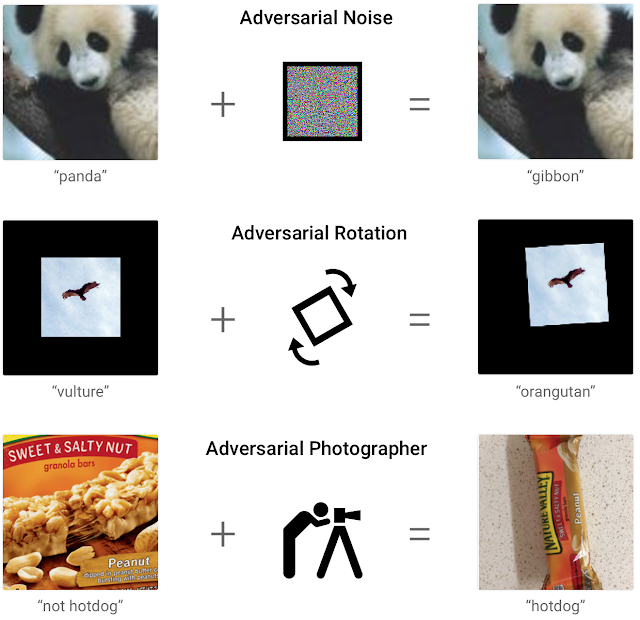
\includegraphics[width=0.75\columnwidth]{figures/unrestricted-advx.png}
	\caption{Unrestricted adversarial examples~\cite{brown2018unrestricted}.}
	\label{fig:unrestricted}
\end{figure}

\begin{figure}
	\centering
	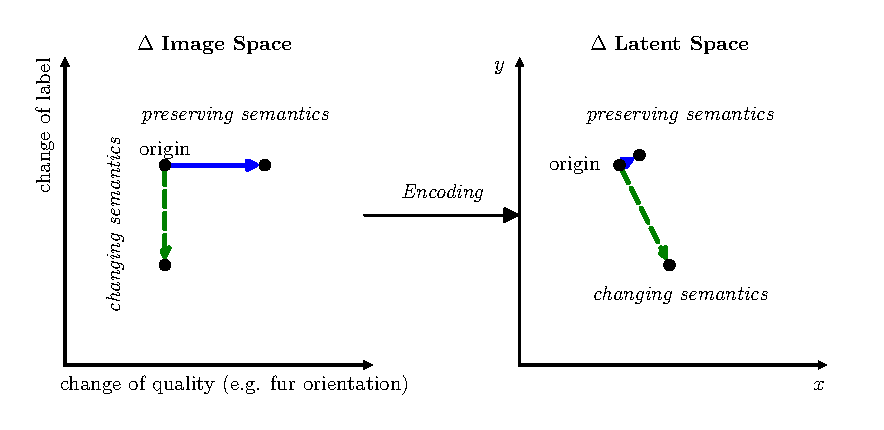
\includegraphics[width=1\columnwidth]{figures/latentspace.pdf}
	\caption{Semantics preserving/changing perturbations in pixel/latent-space (assuming full accuracy).}
	\label{fig:latentspace}
\end{figure}

\begin{figure}[th]
	\centering
	\begin{minipage}[t]{0.24\textwidth}\centering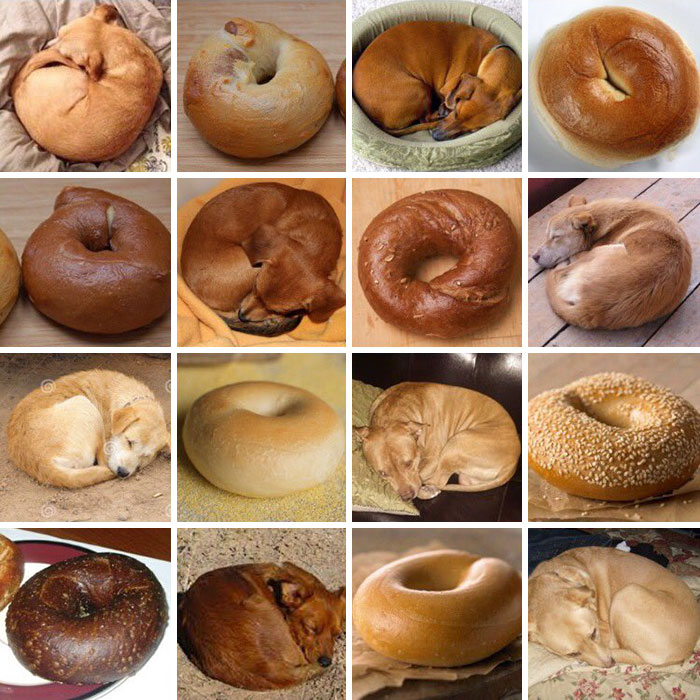
\includegraphics[width=\textwidth]{figures/dog-vs-bagel.jpeg}\end{minipage}
	\hfill
	\begin{minipage}[t]{0.24\textwidth}\centering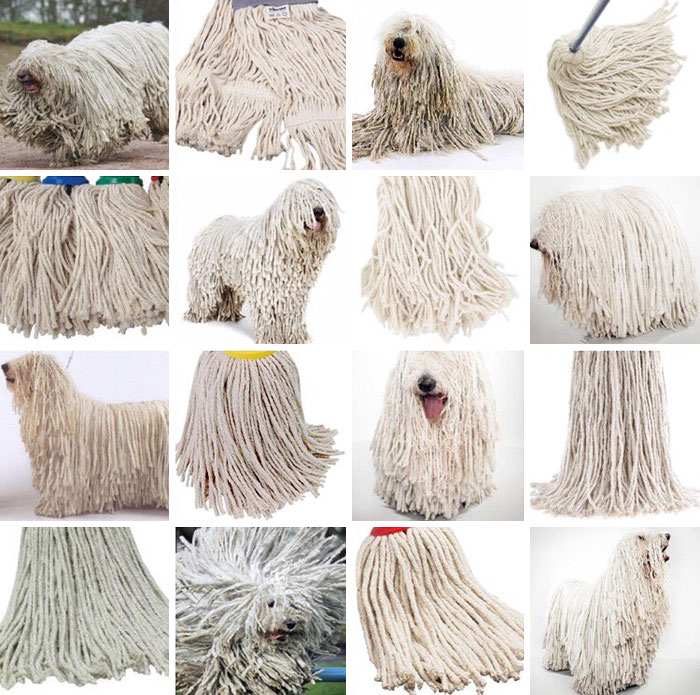
\includegraphics[width=\textwidth]{figures/dog-vs-mop.jpeg}\end{minipage}
	\hfill
	\begin{minipage}[t]{0.24\textwidth}\centering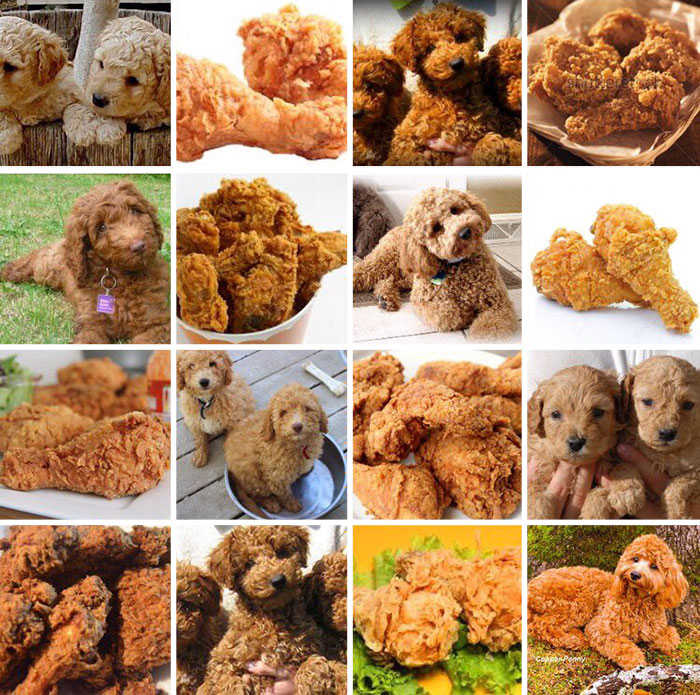
\includegraphics[width=\textwidth]{figures/dog-vs-chicken.jpeg}\end{minipage}
	\hfill
	\begin{minipage}[t]{0.24\textwidth}\centering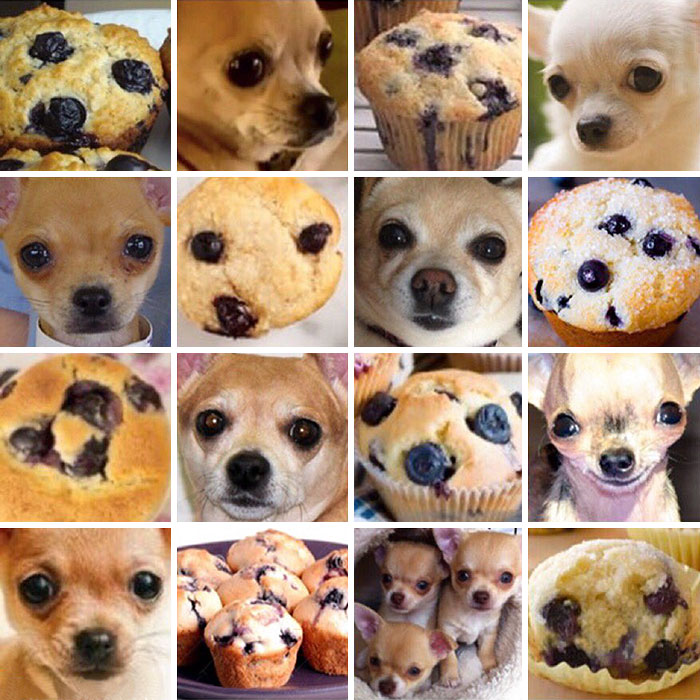
\includegraphics[width=\textwidth]{figures/dog-vs-muffin.jpeg}\end{minipage}
	
	\vspace{1em}

	\begin{minipage}[t]{0.24\textwidth}\centering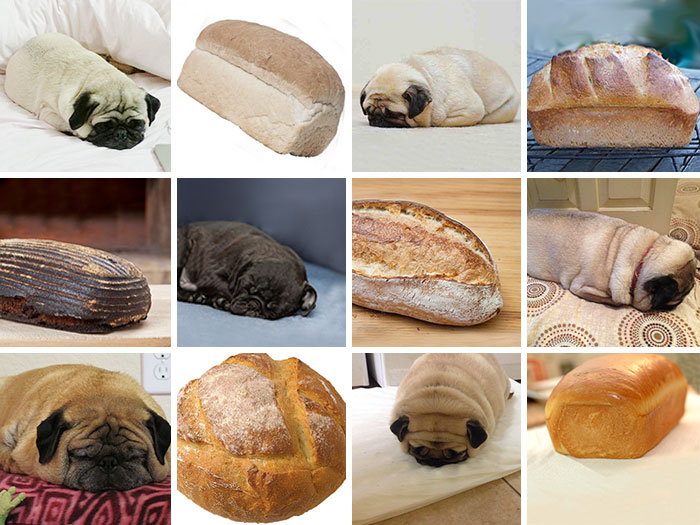
\includegraphics[width=\textwidth]{figures/dog-vs-loaf.jpeg}\end{minipage}
	\hfill
	\begin{minipage}[t]{0.24\textwidth}\centering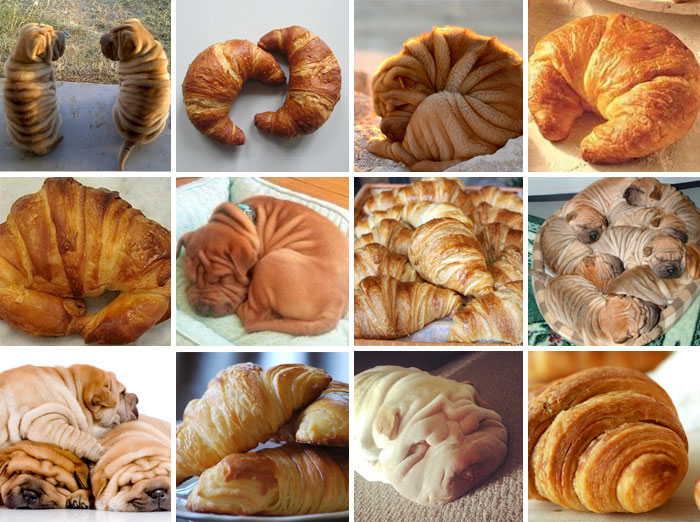
\includegraphics[width=\textwidth]{figures/dog-vs-crossaint.jpeg}\end{minipage}
	\hfill
	\begin{minipage}[t]{0.24\textwidth}\centering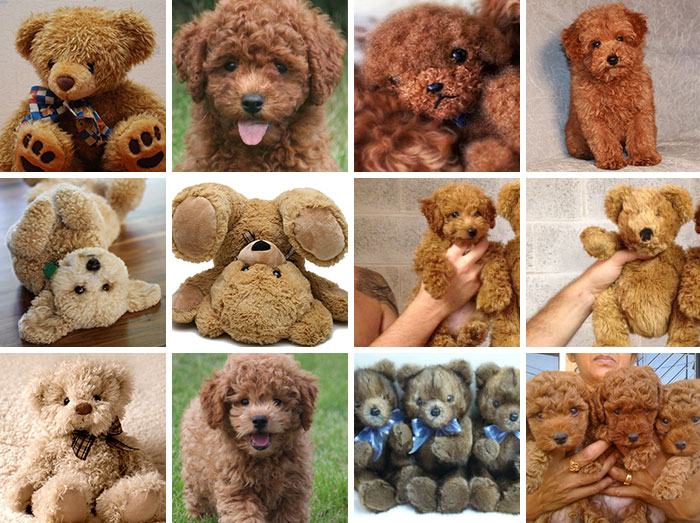
\includegraphics[width=\textwidth]{figures/dog-vs-bear.jpeg}\end{minipage}
	\hfill
	\begin{minipage}[t]{0.24\textwidth}\centering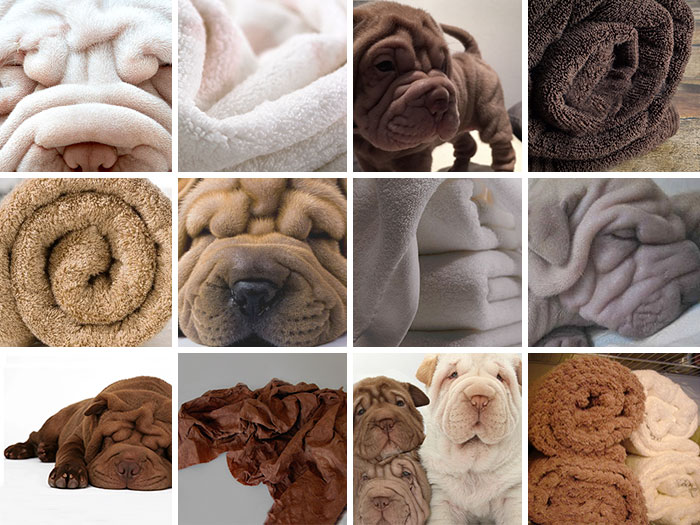
\includegraphics[width=\textwidth]{figures/dog-vs-towel.jpeg}\end{minipage}
	\caption{Natural adversarial examples~\cite{teenybiscuittweet}: Dog vs. Similar looking objects.}
	\label{fig:adversarial_dogs}
\end{figure}

\section{Motivation}

\begin{quotebox}
	\begin{flushright}
		\textit{``The [...] mistake is that you connect that inscrutable thing to important real life things like financial markets or criminal justice systems.''}
		\vspace{1em}

		\textit{``So did you know that AI is being used to perform risk assessments of criminal defendants to decide things like bond amounts or whether somebody gets parole instead of jail? Did you know that machine learning is being used to determine whether people qualify for loans or for mortgages? Did you know that people are using AI to screen job applicants and to match buyers and sellers in equities markets? And of course, as everyone in this room knows, AI is also being used to detect anomalies in cybersecurity settings.''}
		\vspace{1em}

		\textemdash{} James Mickens, USENIX'18~\cite{218395}
	\end{flushright}
\end{quotebox}

One particularly entertaining example of an adversarial attack is the subversion of the conference paper-reviewer assignment model by Eisenhofer et al.~\cite{eisenhofer2023no}, where authors preselect reviewers to gain a competitive advantage.

But adversarial attacks are not limited to academia. Machine learning security has become particularly critical as models are deployed in increasingly sensitive and safety-critical applications~\cite{10585001, ifci2023AnalysisOT, 9099439, Khadka2022ResilientML, yilmaz2021privacy, apruzzese2023real, kumar2020legal, Cao2020HateGANAG, Nurseitov2022ApplicationOM, Zolotukhin2022AttacksAM, huggingface2024security}.

National infrastructure and cyber-physical systems are commonly use machine learning-based protection systems, which can be compromised~\cite{Moradpoor2023TheTO, Chevardin2023AnalysisOA, Ulybyshev2021TrustworthyDA, Halak2022TowardsAP, Rudolph2008DevelopingPS}. A single failure in a nuclear power plant or a water treatment facility or any other critical infrastructure can have catastrophic consequences.

Adversarial attacks can also compromise credit card fraud detection systems, potentially leading to billions in annual losses~\cite{Gu2022DeepLT, Agarwal2021BlackBoxAE, Tsai2024EffectiveAE}.

In healthcare, malicious actors can manipulate medical imaging systems used for diagnosing conditions like skin cancer and Alzheimer's disease, potentially leading to incorrect diagnoses and treatment decisions~\cite{jogani2022analysis, najafi2024dft}. The vulnerability extends to pandemic management systems, where deep learning algorithms processing data from medical IoT devices, including CT scans and thermal cameras, can be compromised through perturbations~\cite{9154468}.

In autonomous vehicles roadside billboards can be weaponized to display specially crafted videos that manipulate vehicle controllers into performing dangerous maneuvers, such as unexpected lane changes or road departures~\cite{Patel2019AdaptiveAV}. Even more concerning, acoustic attacks can exploit image stabilization hardware to create blurred images that cause object detection systems to misclassify or completely miss critical obstacles~\cite{Ji2021PoltergeistAA}. These vulnerabilities are increasing in sophistication~\cite{Axelrod2017CybersecurityCO}.

This risk is also demonstrated in cybersecurity applications, where phishing website detectors face degradation of 3-10\% from realistic evasion attempts that are both cheap and practical to implement~\cite{Yuan2023MultiSpacePhishET}. In the domain of malware detection mutation systems that combine generative networks with reinforcement learning to create metamorphic malware capable of evading detection systems~\cite{to2023effectiveness}.

This has lead to major companies investing heavily in adversarial machine learning research and security.

Microsoft has taken a leading position, spending over \$20 billion on cybersecurity initiatives, with a significant portion dedicated to machine learning security research and their specialized ML red team operations~\cite{coursera_adversarial_2024}.

Open Philanthropy has provided \$330,000 and \$343,235~\cite{openphil2024adversarial} in funding to Carnegie Mellon University dedicated to AdvX research.

The MITRE corporation is now cooperating with Microsoft, Bosch, IBM, NVIDIA, Airbus, Deep Instinct and PricewaterhouseCoopers to develop the Adversarial Machine Learning Threat Matrix~\cite{mitre2024ml} for threat modeling and risk assessment.

The Defense Advanced Research Projects Agency (DARPA) has granted nearly \$1 million to the CV AdvX team at UC Riverside~\cite{roy2020darpa}.
Booz Allen Hamilton, the largest provider of machine learning services for the Federal government, invested in HiddenLayer, Robust Intelligence~\cite{robustintelligence2024, cai2020robust} Shift5, Credo, Hidden Level, Latent, Synthetaic and Reveal Technology~\cite{boozallen2023adversarial, boozallen2023adversarialother}, all of which are dedicated to machine learning security and robustness research.

These investments demonstrate the growing recognition of the importance of protecting machine learning systems from adversarial attacks.

\section{Threat Modeling}

Having established the general concept of adversarial examples, we can now explore the various ways they can be categorized. Our system is not exhaustive: The field continues to evolve, with new attack vectors emerging regularly~\cite{Khaleel2024AdversarialAI}. This is particularly important in threat modeling, where the goal is to anticipate and defend against potential attacks.

We can differentiate between white-box and black-box attacks. White-box attacks assume complete knowledge of and access to the target model, while black-box attacks operate with limited or no access to the model's internal workings~\cite{capozzi2024adversarial}. Interestingly, research has shown that in some cases, black-box attacks can be more effective than white-box approaches at compromising model security~\cite{capozzi2024adversarial}.

An attack can be targeted or untargeted. Targeted attacks aim to manipulate the model into producing a specific, predetermined output, whereas untargeted attacks simply seek to cause any misclassification or erroneous output~\cite{capozzi2024adversarial, Kashyap2024AdversarialAA}. This distinction is particularly relevant in security-critical applications, where the attacker's goals may vary from causing general disruption to achieving specific malicious outcomes.

The method used to generate adversarial examples can be gradient-based, optimization-based or search-based strategies. For example, some text-based attacks leverage language models to generate alternatives for masked tokens, ensuring grammatical correctness and semantic coherence~\cite{garg2020bae}.

The extent to which adversarial examples are transferable \textendash{} meaning their ability to fool multiple different models, or the human vision system\cite{elsayed2018adversarial} \textendash{} is another way to differentiate them. Some adversarial examples demonstrate high transferability across various model architectures, while others are more model-specific in their effectiveness~\cite{Li2022ASO, li2022review}. Recent research has shown that adversarial examples are more readily transferable between vanilla neural networks than between defended ones~\cite{li2019nattack, zheng2023black}.

Finally, attacks can either focus on preserving the semantic meaning of inputs or exploit the mathematical properties of models without regard for semantic interpretation~\cite{browne2020semantics}.

\section{Latent Representations}

The internal latent representations of neural networks, their alignment with human understanding and the resuling gap between the two (the human-machine vision gap~\cite{geirhos2021partial}) is a central theme in adversarial machine learning research. This gap has many practical implications for the robustness and interpretability of machine learning models.

Neural networks trained with topological features develop substantially different internal representations compared to those trained on raw data, though these differences can sometimes be reconciled through simple affine transformations~\cite{mcguire2023neural}. This finding suggests that while the structural representations may differ, the underlying semantic understanding might be preserved across different training approaches.

The Centered Kernel Alignment (CKA) metric enables us to compare neural network representations, though it comes with important caveats. In biological and artificial neural networks, CKA can show artificially high similarity scores in low-data, high-dimensionality scenarios, even with random matrices~\cite{murphy2024correcting}. This limitation is particularly relevant when comparing representations of different sizes or when analyzing specific regions of interest.

The relationship between network architecture and concept representation has also been explored. Generally higher-level concepts are typically better represented in the final layers of neural networks, while lower-level concepts are often better captured in middle layers~\cite{Agafonov2022AnEO, Agafonov2022LocalizationOO}. This hierarchical organization mirrors our understanding of human cognitive processing and suggests that neural networks naturally develop structured representations that align with human conceptual understanding.

The choice of objective function significantly influences how networks represent information, particularly when dealing with biased data. Networks trained with Negative Log Likelihood and Softmax Cross-Entropy loss functions demonstrate comparable capabilities in developing robust representations~\cite{bangaru2022interpreting}.

Recent research~\cite{bansal2021revisiting} has demonstrated that neural networks with strong performance tend to learn similar internal representations, regardless of their training methodology. Networks trained through different approaches, such as supervised or self-supervised learning, can be effectively ``stitched'' together without significant performance degradation. This suggests a convergence in how successful neural networks represent information.

This aligns with the ``Platonic Representation Hypothesis''~\cite{huh2024platonic}, which suggests that neural networks are converging toward a shared statistical model of reality, regardless of their training objectives or architectures. As models become larger and are trained on more diverse tasks and data, their internal representations increasingly align with each other, even across different modalities like vision and language. This convergence appears to be driven by the fundamental constraints\footnote{Formally: ``If an optimal representation exists in function space, larger hypothesis spaces are more likely to cover it.''} of modeling the underlying structure of the real world, similar to Plato's concept of an ideal reality that exists beyond our sensory perceptions. The hypothesis proposes that this convergence is not coincidental but rather a natural consequence of different models attempting to capture the same underlying statistical patterns and relationships that exist in reality~\cite{huh2024platonic}. 

Should the ``Platonic Representation Hypothesis'' hold true, this would either mean that (a) adversarial examples as we know them are misalignments from a converged model of reality, or (b) that there exist a universal adversarial example that can fool any model, regardless of its architecture, training data or objective function, converging to a single and shared model of reality.

Recent work by Moosavi-Dezfooli et al.\ \cite{moosavi2017universal} have demonstrated the existence of a single perturbation that can fool most models for all naturally occurring images, adding weight to the latter interpretation, though the question remains open.

\section{Mental Models}

The question discussed in the previous section is just one of many that remain open and yet have to be fully explained~\cite{shamir2021dimpled}. Among them are:

\begin{itemize}
	\setlength\itemsep{0em}
	\item What are adversarial examples?
	\item Why are the adversarial examples so close to the original images?
	\item Why don't the adversarial perturbations resemble the target class?
	\item Why do robustness and accuracy trade-off~\cite{zhang2019theoretically}?
	\item Why do adversarial examples transfer between models, even on disjoint training sets~\cite{szegedy2013intriguing}?
	\item Why do adversarial examples transfer between models~\cite{szegedy2013intriguing}?
	\item Why do adversarial examples transfer between models and time-limited humans~\cite{elsayed2018adversarial}?
\end{itemize}

Initially, when Szegedy et al.\ \cite{szegedy2013intriguing} coined the term they proposed that adversarial examples are caused by (1) neural networks developing internal representations that become increasingly disconnected from the input features as they progress through deeper layers and (2) that these networks fail to maintain the smoothness properties typically assumed in traditional machine learning approaches. The idea was that this lack of smoothness gives them their expressive power, but also makes them vulnerable to these attacks.

\begin{highlightbox}
	\textbf{Definition:} Manifold \\
	
	The first attempt to explain adversarial examples by Szegedy et al.\ \cite{szegedy2013intriguing} used the term ``manifold'', while refering to a data submanifold. \\
		
	A manifold can be thought of as a low-dimensional structure embedded in a high-dimensional space, representing the set of valid data points (e.g., natural images) that the neural network is trained to classify. Mathematically, if the input data lies on a manifold $\mathcal{M} \subset \mathbb{R}^m$, then $\mathcal{M}$ represents the subset of the high-dimensional input space $\mathbb{R}^m$ that corresponds to meaningful or real-world data. \\

	Szegedy et al.\ suggest that adversarial examples exploit the structure of this manifold and its surrounding space. Specifically, adversarial examples are small perturbations $r$ added to an input $x \in \mathcal{M}$, such that the perturbed input $x' = x + r$ lies off the data manifold but still within the high-dimensional input space. \\
	
	Formally, given a classifier $f: \mathbb{R}^m \to \{1, ..., k\}$ and its associated loss function $\text{Loss}_f(x, y)$, an adversarial example $x'$ for an input $x$ with true label $y$ can be found by solving:
	
	$$\min_{r} \|r\|_2 \quad \text{subject to } f(x + r) \neq y, \; x + r \in [0, 1]^m$$
	
	where $r$ is constrained to be small (e.g., in terms of its $L_2$-norm). This optimization problem effectively traverses the space near $x$, moving off the manifold $\mathcal{M}$, to find regions where the classifier's decision boundary behaves unexpectedly. \\
	
	The paper suggests that these adversarial examples expose ``blind spots'' in the learned representation of the manifold by the neural network. The network's decision boundary may extend into regions near $\mathcal{M}$ in ways that are not semantically meaningful, allowing adversarial perturbations to exploit these regions. This phenomenon arises due to the high dimensionality of the input space and the discontinuous mappings learned by deep networks, which can fail to generalize smoothly beyond the manifold~\cite{khoury2018geometry, Jha2018DetectingAE, Sha2020ADA, dube2018high, shamir2021dimpled}. \\
	
	A more rigorous definition of the manifold hypothesis is provided by Khoury et al.\ \cite{khoury2018geometry}.
\end{highlightbox}

\begin{highlightbox}
	\textbf{Definition:} Realism  \\

	A ``realistic subspace'' can be understood as a subset of the data manifold where the images appear plausible according to human perception or a given distribution $P$. A simple formula that expresses this idea elegantly to quantify realism is derived from the notion of randomness deficiency in algorithmic information theory~\cite{theis2024makes}:

	$$U(x) = -\log P(x) - K(x)$$

	where $P(x)$ is the probability density of the image $x$ under the target distribution and $K(x)$ is the Kolmogorov complexity of $x$, representing the shortest description of $x$ in a universal programming language. This measure, called a ``universal critic'', captures how well $x$ aligns with both the statistical properties of $P$ and its compressibility. A low value of $U(x)$ indicates that $x$ is realistic, while a high value suggests it is unrealistic~\cite{theis2024makes}. \\

	This approach generalizes prior methods by integrating both probabilistic and structural aspects of realism. It highlights that realism depends not only on adherence to statistical patterns (e.g., probabilities or divergences) but also on whether an image can be plausibly generated within the constraints of $P$. While directly computing $K(x)$ is infeasible due to its uncomputability, practical approximations (e.g., compression algorithms or neural network-based critics) can serve as proxies~\cite{theis2024makes}. \\

	The distinction between realistic and unrealistic perturbations is crucial for practical applications, as some adversarial examples may be mathematically valid but physically impossible to realize in real-world scenarios~\cite{dyrmishi2023empirical}. \\
	
	The challenge of quantifying realism remains a fundamental problem in machine learning~\cite{theis2024makes}.
\end{highlightbox}

Since then there have been many attempts at finding a cohesive narrative to explain these counter-intuitive properties, each with their own limitations and assumptions \textendash{} some complementary, some contradictory~\cite{ilyas2019adversarial}.

\paragraph{Non-robust features \& concentration of measure in high-dimensions.} Most popularly, Ilyas et al.\ \cite{ilyas2019adversarial} proposed that features that models learn from can be divided in 3 categories: (1) useless featurs, to be discarded by the feature extractor, (2) robust features, which are comprehensible to humans, generalize across multiple datasets and remain stable under small adversarial perturbations and (3) non-robust features, which are incomprehensible to humans, learned by the supervised model to exploit patterns in the data distribution which are highly effective for the task at hand but also brittle and easily manipulated by adversarial perturbations. The authors suggest that the vulnerability of deep neural networks to adversarial examples is due to their reliance on non-robust features and inherent to how the models are optimized to minimize the loss function. In essence, the authors argue that adversarial vulnerability is a property of the dataset, not the algorithm and by removing these non-robust features from the training data although the adversarial robustness of the model can be improved, due to information loss of the most predictive features, the model's overall accuracy will decrease. This view is also shared among~\cite{engstrom2019a, raghunathan2018certified, wong2018provable, xiao2018training, cohen2019certified, fawzi2018adversarial, mahloujifar2019curse, shafahi2018adversarial, gilmer2018adversarial, madry2017towards}.

\paragraph{Theoretical constructions which incidentally exploit non-robust features.} A complimenting hypothesis is that because models trained to maximize accuracy will naturally utilize non-robust data, regardless of whether it aligns with human perception~\cite{ilyas2019adversarial} they add a low-magnitude weight to sensitive variables that can get overamplified by adversarial examples~\cite{bubeck2019adversarial, nakkiran2019adversarial}. The assumption is that this happens due to computational constraints or model complexity.

\paragraph{Insufficient data.} Schmidt et al. argue~\cite{schmidt2018adversarially} that adversarial vulnerabilities are intrinsic to statistical learning in high-dimensional spaces and not merely due to flaws in specific algorithms or architectures. This is a natural consequence of the mental model proposed by Ilyas et al.\ \cite{ilyas2019adversarial}. They also argue that due to information loss in a robust dataset, significantly more data is required during training in order to achieve comparable performance.

\paragraph{Boundary Tilting.} A competing view by Tanay and Kim et al.\ \cite{tanay2016boundary,kim2019bridging} suggests that adversarial examples exist because decision boundaries extend beyond the actual data manifold and can lie uncomfortably close to it, essentially viewing adversarial examples as a consequence of overfitting. This observation can be quantified through the concept of adversarial strength, which relates to the angular deviation between the classifier and the nearest centroid classifier. The authors also argue that this vulnerability can be addressed through proper regularization techniques.

\paragraph{Test Error in Noise.} There might be a link between robustness to random noise and adversarial attacks~\cite{fawzi2016robustness, lecuyer2019certified, cohen2019certified, ford2019adversarial}. This might imply that adversarial examples exploit inherent weaknesses in how models generalize under noisy or perturbed conditions.

\paragraph{Local Linearity.} Goodfellow, Shlens and Szegedy et al.\ \cite{goodfellow2014explaining, madry2017towards} argue that even though DNNs are highly nonlinear overall, their behavior in high-dimensional spaces often resembles that of linear models. This makes the models vulnerable to small, targeted perturbations similar to how they are computed by FGSM. However some adversarial examples are successful all while defying the assumption of local linearity and reducing a model's linearity does not necessarily improve its robustness either~\cite{athalye2018obfuscated}.

\paragraph{Piecewise-linear decision boundaries.} In the ``dimpled manifold hypothesis''~\cite{shamir2021dimpled} the central claim is that adversarial examples emerge because we attempt to fit high $n-1$ dimensional decision boundaries to inherently low-dimensional data like images (which can be losslessly projected to $k \ll n$ dimensions). This leaves redundant dimensions on which adversarial examples won't be judged, which enables them exist roughly perpendicularly from the true location of the low-dimensional natural image, by using large gradients. In this mental model adversarial examples can be on-manifold or off-manifold, based on the angle of the gradients relative to the data manifold.

The authors also suggest that decision boundaries of neural networks evolve during training. This happens through two distinct phases. First, there is a rapid ``clinging'' phase where the decision boundary moves close to the low-dimensional image manifold containing the training examples. This is followed by a slower ``dimpling'' phase that creates shallow bulges in the decision boundary, pushing it to the correct side of the training examples, without shifting the plane. This gradient descent based process is highly efficient, but it also leaves a brittle decision boundary that can be easily exploited.

This implies that any attempt to robustify a network by limiting all its directional derivatives will make it harder to train and thus less accurate.

It also explains why networks trained on incorrectly labeled adversarial examples can still perform well on regular test images, as the main effect of adversarial training is simply to deepen these dimples in the decision boundary.

Lukas Karner successfully was able to successfully reproduce the experiments from the ``Dimpled Manifold Hypothesis'' paper in 2023~\cite{karner2023dimpled}. He additionally demonstrated that dimensionality reductions increases the interpretability of the perturbations to humans~\cite{karner2023dimpled}.

However, despite the experiments being carried out correctly themselves, the chain of reasoning might be flawed, as shown by a succinct (<100 LoC) counterexample by Yannik Kilcher in 2021~\cite{kilcher2021dimpledcode, kilcher2021dimpled}. While the ``Dimpled Manifold Hypothesis'' implies a relatively uniform vulnerability across all dimensions the counterexperiment contradicts these assumptions through successful adversarial attacks constructed by perturbing either an arbitrary subset of selected dimensions or their complement. If the decision boundary truly ``clung'' to the data manifold, restricting perturbations to a subset of dimensions would not have produced successful adversarial examples. The ability to generate adversarial examples in complementary subspaces suggests the decision boundary structure is more complex than just simple dimples.

To summarize, there is no consensus on the root cause of adversarial examples and the field remains an active area of research. The mental models proposed by different researchers are not necessarily mutually exclusive and it is likely that the true explanation involves a combination of these factors.

\section{Defenses}

Having discussed the various theories and approaches in explaining adversarial examples, we can now turn our attention to the countermeasures that have been proposed to mitigate their impact.

\subsection{Train- and Test-time defenses}

A leaderboard of adversarial robustness can be found on the RobustBench platform~\cite{croce2021robustbench}, which provides a standardized evaluation of adversarial robustness across a wide range of models and datasets. The platform includes a variety of metrics for evaluating robustness, such as the $\ell_\infty$ and $\ell_2$ adversarial perturbation sizes, as well as the robust accuracy under different attack settings.

Several effective strategies have been developed. This collection is by no means exhaustive.

\paragraph{Adversarial Training.} One of the least invasive methods to improve adversarial robustness is adversarial training. Incorporating adversarial examples into the training process improves model resilience by learning from potential attack patterns and helps maintain performance on clean data~\cite{araujo2020advocating, Ren2022VulnerabilityAR}. However, this requires the anticipated attacks to be known in advance. An alternative would be introducing derived variables for controlled randomness to input data during training, which is still effective~\cite{Adeke2023SecuringNT}.

\paragraph{Quality Assessment Integration.} Implementing image quality assessment combined with knowledge distillation helps detect potentially harmful inputs that could cause incorrect model predictions~\cite{feng2020towards}. Another alternative preprocessing technique is using brain inspired encoders~\cite{Rakhimberdina2022StrengtheningRU}. This method is particularly effective as it doesn't require model retraining, but depending on the preprocessing techique used, it can be computationally expensive.

\paragraph{Moving Target Defense.} Using heterogeneous models, diversifying the model structure, using ensembles and dynamic model switching can protect against white-box adversarial attacks. This approach will make attack vectors that work on one model ineffective on others~\cite{Li2023wAdvMTDAM}.

\paragraph{Statistical Detection.} Statistical tests can be employed for some signal based deep learning systems to detect adversarial examples. This includes analyzing peak-to-average-power ratio and examining softmax outputs of the model~\cite{KokaljFilipovic2019AdversarialEI}.

\paragraph{Enhanced Transformation.} Transformation-based defense strategies, such as using generative adversarial networks (GANs), can help recover from adversarial examples. These methods can counteract adversarial effects while maintaining or even improving classification performance~\cite{Zhao2023EITGANAT}.

The countermeasures discussed so far provide a diverse array of techniques to mitigate the impact of adversarial examples. Each method addresses specific aspects of the problem, ranging from input preprocessing to model architecture adjustments and training methodologies. Notably, hybrid strategies that combine multiple techniques often yield the best results, with some implementations achieving reliable performance even under sophisticated attack benchmarks~\cite{ji2023benchmarking}.

\subsection{Architectural Defenses}

Assuming that robustness and generalizability are not competing objectives but complementary goals, the ultimate defense lies in designing architectures that inherently integrate robustness and interpretability. By prioritizing these objectives at the core of model development, we can create systems that not only withstand adversarial attacks but also offer more trustworthy and transparent decision-making.

\paragraph{Fermi-Bose Machine.} One noteworthy example is the Fermi-Bose Machine~\cite{xie2024fermi}. Unlike traditional neural networks that rely on backpropagation, this method introduces a local contrastive learning mechanism inspired by quantum mechanics principles. The system works by making representations of inputs with identical labels cluster together (like bosons), while representations of different labels repel each other (like fermions). This layer-wise learning approach is considered more biologically plausible than traditional backpropagation~\cite{xie2024fermi}. The researchers demonstrated the effectiveness of their method on the MNIST dataset, showing that by adjusting the target fermion-pair-distance parameter, they could significantly reduce the susceptibility to adversarial attacks that typically disturb standard perceptrons~\cite{xie2024fermi}. The key innovation lies in controlling the geometric separation of prototype manifolds through the target distance parameter, as revealed by statistical mechanics analysis~\cite{xie2024fermi}.

\paragraph{Ensemble everything everywhere.} A recent (August 2024) state-of-the-art approach works by multi-resolution input representations and dynamic self-ensembling of intermediate layer predictions~\cite{fort2024ensemble}. The researchers introduced a robust aggregation mechanism called CrossMax, based on Vickrey auction, which combines predictions from different layers of the network~\cite{fort2024ensemble}.

The method achieved impressive results without requiring adversarial training or additional data, reaching approximately 72\% adversarial accuracy on CIFAR-10 and 48\% on CIFAR-100 using the RobustBench AutoAttack suite~\cite{fort2024ensemble}. When combined with simple adversarial training, the performance improved further to 78\% on CIFAR-10 and 51\% on CIFAR-100, surpassing the current state-of-the-art by 5\% and 9\% respectively~\cite{fort2024ensemble}.

An interesting secondary outcome of this research was the discovery that gradient-based attacks against their model produced human-interpretable images of target classes~\cite{fort2024ensemble}. Additionally, the multi-resolution approach enabled the researchers to transform pre-trained classifiers and CLIP models into controllable image generators, while also developing successful transferable attacks on large vision language models~\cite{fort2024ensemble}.

\section{Future Directions}

Perhaps we should be rethinking unrestricted adversarial examples not as attacks but as indicators of insufficient generalization, which can not always be measured by accuracy on a predefined test set alone.

The most promising path forward may not lie in defending against these examples, but rather in fundamentally reimagining model architectures with reliability, robustness and interpretability as core design principles. This way, robustness becomes a natural byproduct of the model's structure, at no additional cost.

This perspective suggests that enhancing adversarial robustness requires developing new architectures from the ground up that inherently exhibit these properties, rather than patching existing systems.

\chapter{Methodology \& Results}

\begin{quotebox}
	\begin{flushright}
		\textit{``Well, at a high level, I think that the goal of computer security is to ensure that systems do the right thing, even in the presence of malicious inputs. Now, achieving this goal in the context of machine learning is exceptionally challenging for two reasons. [...] So first of all, computer scientists lack a deep mathematical understanding of how machine learning actually learns and predicts. [...] And second, many people who deploy machine learning don't actually care about the first problem.''}
		\vspace{1em}

		\textit{``And if somebody asks you why the stuff worked, you just say the stuff is what the stuff is brother, accept the mystery. Okay. And so basically machine learning is like this, right? So we've invented, invented a bunch of techniques that kind of work, like in some cases, but we're not really sure what's going on. [...] We don't ask questions about the weights. We just wake up, we go to work, we use the weights, we go back home. Okay. If we change the weights, the predictions would be different and less good, probably... depending on the weather... so we don't ask about the weights.''}
		\vspace{1em}

		\textemdash{} James Mickens, USENIX'18~\cite{218395}
	\end{flushright}
\end{quotebox}

When studying unrestricted adversarial examples in computer vision, we are essentially dealing with a black box. Top-performing models are all deep neural networks, which are notoriously hard to interpret. This lack of interpretability means we can't easily pinpoint why these models make certain decisions or more importantly, why they fail. This presents a challenge when trying to understand and mitigate adversarial vulnerabilities.

To address this challenge, we've adopted two guiding principles: (1) keeping it simple by using basic geometric masks to overlay on images, avoiding complex spatial transformations or advanced attack techniques and (2) leveraging intermediary layers of neural networks to enhance interpretability.

% 
% hcaptcha experiments
% 

\section{HCaptcha Inspired Geometric Masks}

\subsection{Research Motivation}

We noticed a gap in research when it comes to unrestricted adversarial examples that exploit the human-machine vision gap. One practical application for these types of attacks is in developing robust CAPTCHAs\footnote{Completely Automated Public Turing test to tell Computers and Humans Apart}, which are widely used to differentiate between humans and bots. The aim is to create images that machines struggle or ideally fail to recognize, while remaining easily solvable by humans.

The biggest advantage of using CAPTCHAs for adversarial research is their proven effectiveness. By studying the challenges of top providers like Google's reCAPTCHA and hCaptcha, we can start off with a strong baseline \textendash{} with a proven track record of robustness \textendash{} to build upon. This saves us from having to reinvent the wheel. Additionally a CAPTCHA challenge is a well-defined problem with clear success criteria and would enable future studies to conduct adversarial research and their transferability to humans on a large scale with significantly fewer ethical, legal and financial constraints.

\begin{figure}
	\centering
	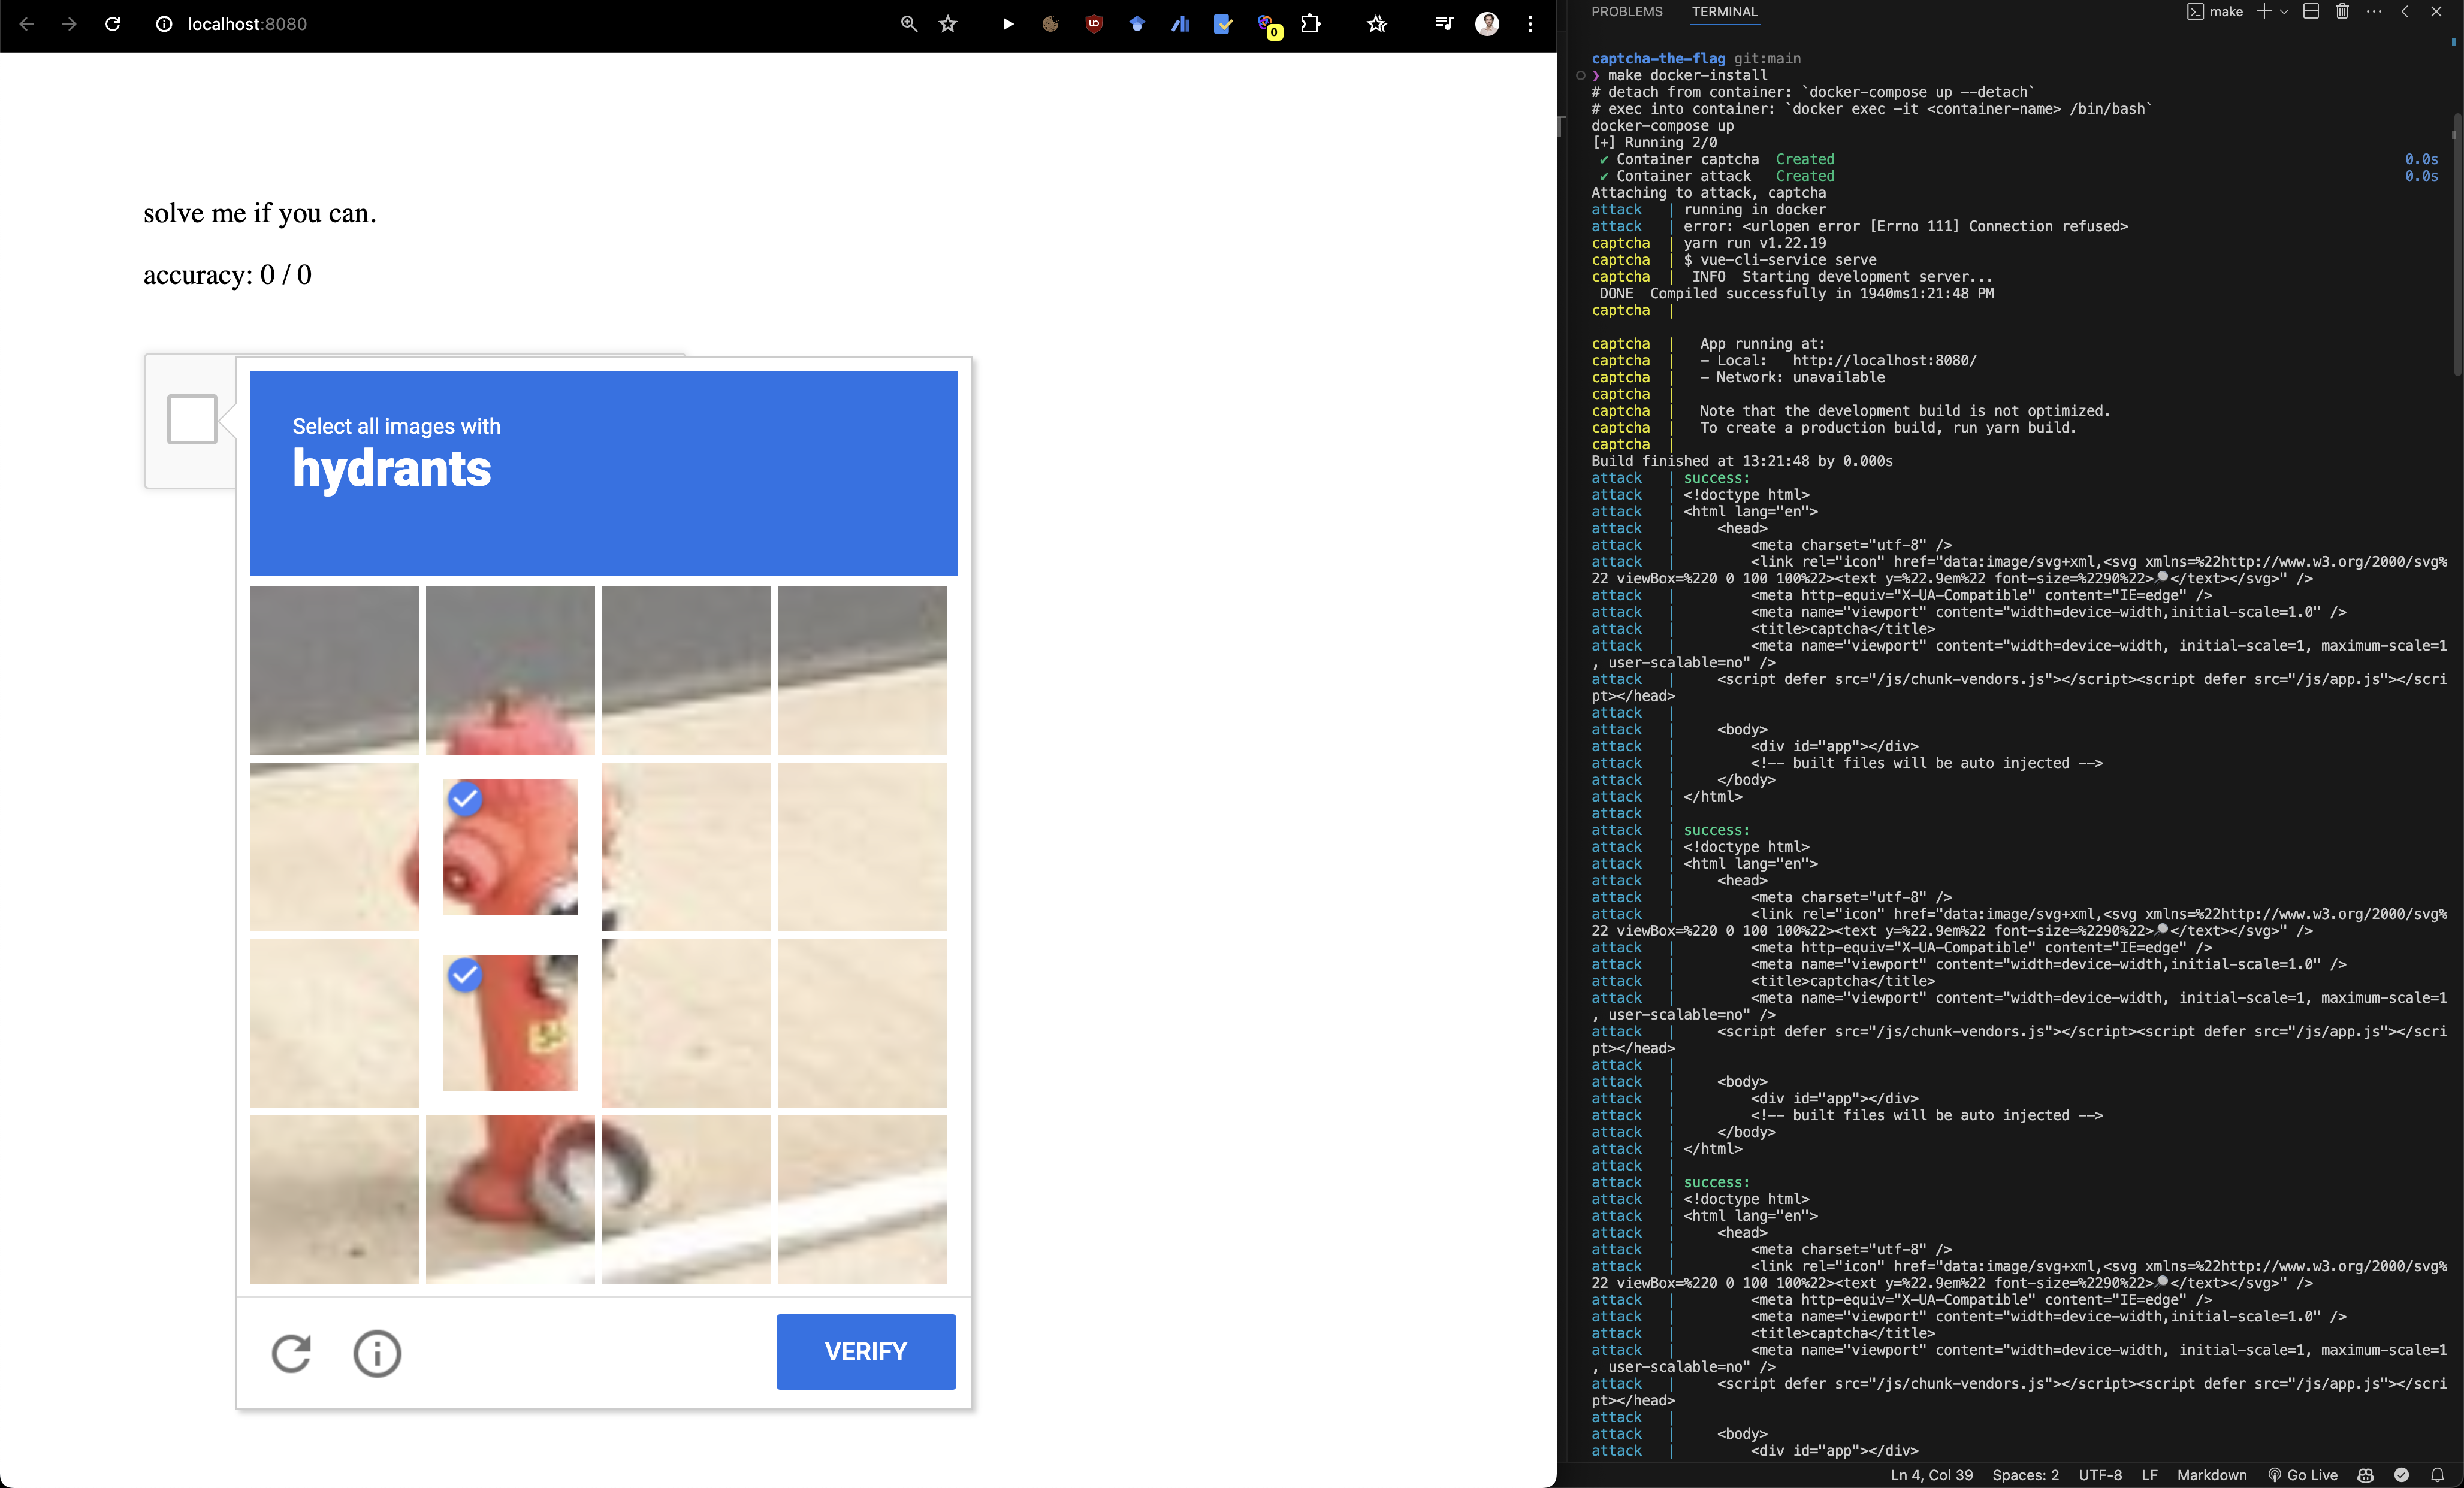
\includegraphics[width=1\columnwidth]{figures/ctf.png}
	\caption{ReCAPTCHAv2 cybersecurity emulation framework \\ \url{https://github.com/ETH-DISCO/captcha-the-flag}}
	\label{fig:ctf}
\end{figure}

A demo, shown in Figure~\ref{fig:ctf}, was built to showcase the potential of adversarial examples in CAPTCHAs and provide an emulation framework of reCAPTCHAv2 for penetration testing purposes. It is composed of two containers responsible for the challenger and the solver, respectively.

The first step in this direction was studying the effectiveness of CAPTCHA solvers for each provider, in the order of their market share.

Despite Google's reCAPTCHA having a global market share of at least 99\%~\cite{authkong2024recaptcha}, they have been shown to be solvable with 100\% accuracy using publicly available computer vision models on consumer hardware, by Plesner et al.~\cite{plesner2024breaking}.

HCaptchas, on the other hand, have remained undefeated in the ongoing attack-defense arms race. In fact, several dedicated open-source communities collaborating on building a solver for hCaptcha report low success rates~\cite{hcaptcha2024base64, hcaptcha_challenger}. This is coupled with our observation on sophisticated defenses being rolled out by hCaptcha on an almost weekly basis. Within the last 6 months we were studying hCaptcha, we observed the obfuscation of metadata and payloads, the introduction of new reasoning-based challenges through question answering and the introduction of new classification and segmentation challenges. This leads us to believe that hCaptcha is the most robust CAPTCHA provider on the market today.

Two hCaptcha challenges were selected for our experiments: a classification challenge and a segmentation challenge. The classification challenge overlays images with simple, predictable patterns like grids of colored geometric shapes (e.g., circles or squares). The segmentation challenge works by overlaying images with more complex patterns, such as a grid of colored geometric shapes with varying sizes and rotations. These challenges are designed to be easily solvable by humans, but difficult for machines to classify accurately.

\begin{highlightbox}
	\textbf{Idea:} Evaluation on Synthetic Data \\

	One interesting idea we explored but ultimately set aside was the use of synthetic images for adversarial training and evaluation of (natural unrestricted) adversarial examples. Although promising, it didn't quite align with our primary goals. We developed a pipeline that chains together several advanced models: starting with stable diffusion to generate an image, then using GPT-2 to caption it. These captions were used as text queries for zero-shot classification and detection models like CLIP and ViT, which perform exceptionally well but need a prompt to work. Finally, we used SAM1 for segmentation. This process is illustrated in Figure~\ref{fig:chained}. This is an exciting direction, especially with the advancements brought by FLUX.1~\cite{BlackForestLabs2024FLUX}, not sufficiently explored in the current literature, based on our preliminary review. \\

\begin{minted}[fontsize=\footnotesize]{python}
img = gen_stable_diffusion("an austronaut on mars riding a horse")
query = caption_gpt2(img)
probs = classify_clip(img, query)
boxes, scores, labels = detect_vit(img, query, 0.1)
masks = segment_sam1(img, boxes)
\end{minted}
\end{highlightbox}

\begin{figure}
	\centering
	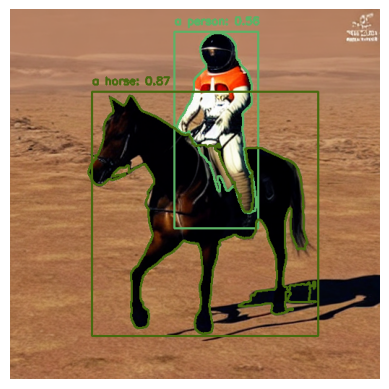
\includegraphics[width=0.3\columnwidth]{figures/chained.png}
	\caption{Evaluation on synthetic data.}
	\label{fig:chained}
\end{figure}

\subsection{Experimental Setup}

The first series of experiments focused on evaluating the performance of state-of-the-art computer vision models on hCaptcha challenges. The goal was to assess the performance of solvers and identify potential vulnerabilities that could be exploited to generate CAPTCHA based adversarial examples. We targeted a single type of challenge: The classification challenge, which involves overlaying images with simple, predictable patterns like grids of colored geometric shapes (e.g., circles or squares).

We also studied and reconstructed the segmentation challenge, which embeds images within a Perlin-noise-like pattern, smooths the edges, adds a slight blur and sometimes incorporates the geometric masks from the classification challenge on either individual segments or the entire image. However, given the number of variables involved, we decided to focus on the classification challenge for our initial experiments and leave the other tasks for future work. Our goal was to establish a reliable baseline, not to exhaustively explore all possibilities. However, we noticed through small-scale experiments using SAM1 and SAM2 that it was significantly more difficult to solve than the classification challenge.

\paragraph{Mask Generation.}

We developed a sublibrary that allows for the parametrizable reconstruction of geometric masks used in the classification task using the rendering engine \texttt{pycairo}. We created four distinct masks to overlay on images at varying intensities: ``Circle'', ``Diamond'', ``Square'' and ``Knit'' (the ``Word'' mask was also reconstructed, but omitted as they have been proven to be easy to mitigate~\cite{zhang2023text,dong2023robust,shayegani2023plug}).

These masks were chosen based on an experiment where we hand-labeled 1600 images from hCaptcha\footnote{Credits to Turlan Kuzhagaliyev.}. The opacities (alpha values) and densities of these masks were determined through an initial hyperparameter search, which we'll discuss later. Figure~\ref{fig:hcaptchacombined} showcases the optimized reconstructions we used to benchmark the models.

For the segmentation task, we experimented with various background textures, including Perlin noise and color-encoded multivariate Gaussian distributions. Figure~\ref{fig:segchallenge} shows both a selected example and its reconstruction. But as mentioned earlier, we decided to focus on the classification challenge for our initial experiments.

\begin{figure}[th]
	\begin{subfigure}[t]{0.19\textwidth}\centering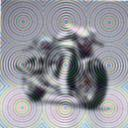
\includegraphics[width=\linewidth]{figures/hcaptcha-circle.png}\caption{``Circle'' mask}\label{fig:subfig1}\end{subfigure}
	\hfill
	\begin{subfigure}[t]{0.19\textwidth}\centering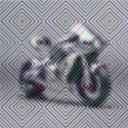
\includegraphics[width=\linewidth]{figures/hcaptcha-diamond.png}\caption{``Diamond'' mask}\label{fig:subfig2}\end{subfigure}
	\hfill
	\begin{subfigure}[t]{0.19\textwidth}\centering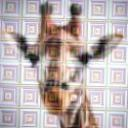
\includegraphics[width=\linewidth]{figures/hcaptcha-square.png}\caption{``Square'' mask}\label{fig:subfig3}\end{subfigure}
	\hfill
	\begin{subfigure}[t]{0.19\textwidth}\centering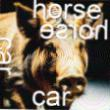
\includegraphics[width=\linewidth]{figures/hcaptcha-word.png}\caption{``Word'' mask}\label{fig:subfig4}\end{subfigure}
	\hfill
	\begin{subfigure}[t]{0.19\textwidth}\centering\phantom{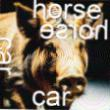
\includegraphics[width=\linewidth]{figures/hcaptcha-word.png}}\end{subfigure}
	
	\begin{subfigure}[t]{0.19\textwidth}\centering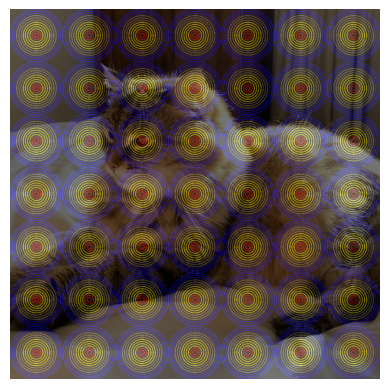
\includegraphics[width=\linewidth]{figures/hcaptcha-copy-circle.png}\caption{``Circle'' mask\\(reconstructed)}\label{fig:subfig5}\end{subfigure}
	\hfill
	\begin{subfigure}[t]{0.19\textwidth}\centering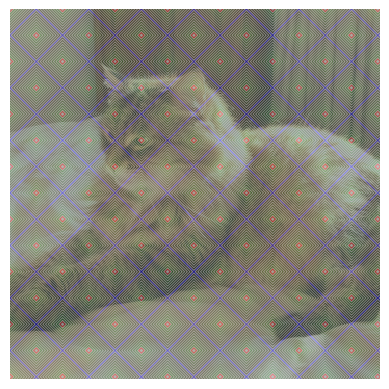
\includegraphics[width=\linewidth]{figures/hcaptcha-copy-diamond.png}\caption{``Diamond'' mask\\(reconstructed)}\label{fig:subfig6}\end{subfigure}
	\hfill
	\begin{subfigure}[t]{0.19\textwidth}\centering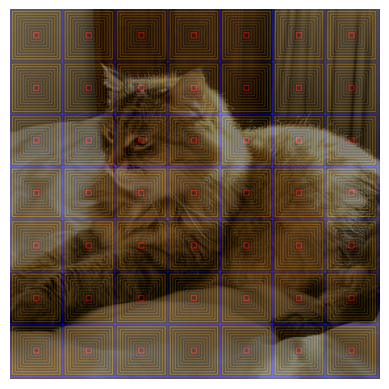
\includegraphics[width=\linewidth]{figures/hcaptcha-copy-square.png}\caption{``Square'' mask\\(reconstructed)}\label{fig:subfig7}\end{subfigure}
	\hfill
	\begin{subfigure}[t]{0.19\textwidth}\centering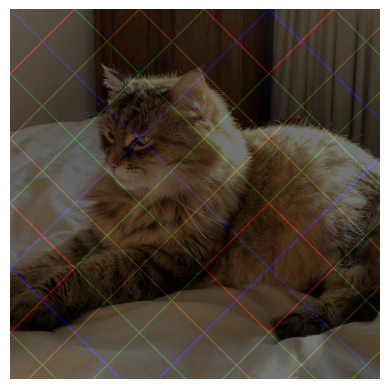
\includegraphics[width=\linewidth]{figures/hcaptcha-copy-knit.png}\caption{``Knit'' mask\\(custom)}\label{fig:subfig8}\end{subfigure}
	\hfill
	\begin{subfigure}[t]{0.19\textwidth}\centering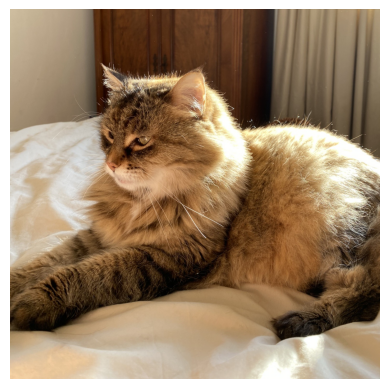
\includegraphics[width=\linewidth]{figures/hcaptcha-copy-original.png}\caption{Original image\\(for reconstructions)}\label{fig:subfig9}\end{subfigure}

	\caption{Selected examples by hCAPTCHA and their optimized reconstructions. The ``Word'' overlay was ommited and replaced with a custom ``Knit'' mask.}
	\label{fig:hcaptchacombined}
\end{figure}

\begin{figure}[th]
	\centering
	\begin{minipage}[t]{0.49\textwidth}\centering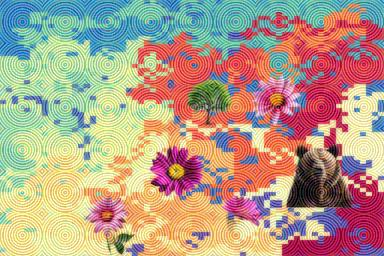
\includegraphics[width=\textwidth]{figures/hcaptcha-seg.png}\caption{Segmentation Challenge.}\label{fig:segchallenge}\end{minipage}
	\hfill
	\begin{minipage}[t]{0.49\textwidth}\centering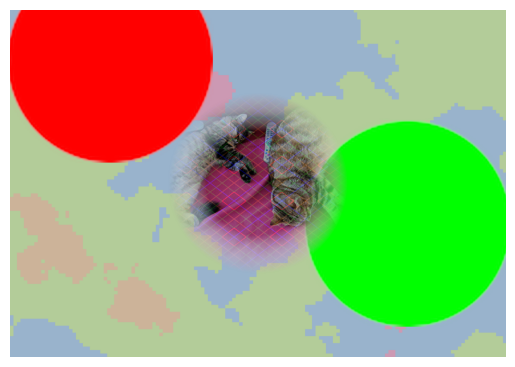
\includegraphics[width=\textwidth]{figures/hcaptcha-seg-baiba.png}\caption{Reconstruction (arbitrary parameters).}\label{fig:segreconstruction}\end{minipage}
\end{figure}

\paragraph{Model Selection.}

To identify the best zero-shot open vocabulary classification, object detection and segmentation models that can run on a consumer hardware, we did a near exhaustive literature review. We looked at focused research papers~\cite{wang2024benchmarking, goldblum2024battle} and checked out public leaderboards from HuggingFace, TIMM, PapersWithCode, Github Trends, Pytorch benchmarks and more. Our goal was to ensure that the solver could break CAPTCHAs on any machine with minimal setup.

After the literature review we clustered the models by their architecture family and clustered them on a scatter plot based on their performance, inspired by~\cite{howard_image_models}. We then selected the top models from each family and attempted to run them on a consumer machine, assuming that they are publicly available. This was to test the feasibility of running these models in a real-world scenario.

We chose several models to test, including ``ConvNeXt\_XXLarge''~\cite{Liu_2022_CVPR}, Open CLIP's ``EVA01-g-14-plus''~\cite{Fang_2023_CVPR} and ``EVA02-L-14''~\cite{fang2024eva}, ``DFN5B-CLIP-ViT-H'' by Apple \cite{fang2023data}, the original ``ViT-L-14-378'' and ``ViT-H-14-378-quickgelu''~\cite{dosovitskiy2021imageworth16x16words}, ``ResNet50x64''~\cite{He_2015_ICCV} and RoBERTa-B and RoBERTa-L~\cite{conneau2020unsupervisedcrosslingualrepresentationlearning}. We highlight results for a subset of these models, specifically ConvNeXt, EVA01, EVA02, ViT-H-14 and ResNet50. These models were picked to cover key architectures in both convolutional and transformer-based approaches, allowing us to see how well our masks work across different architecture families.

We also evaluated a custom adversarially trained ResNet-50, but due to its poor performance, we decided to exclude it from the final results.

\paragraph{Dataset Selection.}

For our experiments, we used the enriched ImageNet dataset with 1,000 entries from ``visual-layer'' on HuggingFace.

\paragraph{Evaluation Metrics.}

To evaluate, we focused on two main aspects: perceptual quality and model accuracy.

Perceptual quality is all about how visually similar the adversarial examples are to the original images. We used a weighted average metric to get a comprehensive view of image quality. This metric combines cosine similarity (15\% weight)~\cite{singhal2001modern}, Peak Signal-to-Noise Ratio (PSNR, 25\% weight)~\cite{9311108}, Structural Similarity Index (SSIM, 35\% weight)~\cite{wang2004image} and Learned Perceptual Image Patch Similarity (LPIPS, 25\% weight)~\cite{lpips}. These weights were chosen to balance the importance of each component in assessing overall image quality. We also used the Fréchet Inception Distance (FID), however it was omitted from the final metric due to its high computational cost. Overall, we want this number to be as high as possible.

On the accuracy front, we looked at how well the models performed in predicting the correct class. The models output a list of classes sorted by likelihood. We measured accuracy using the top-k accuracy metric, specifically accuracy@1 (Acc@1) and accuracy@5 (Acc@5). This tells us how often the correct label is in the top 1 or top 5 predicted classes, respectively. Finally, we calculated the adversarial accuracy (AdvAcc) as the difference in accuracy between adversarial and benign examples. This metric gives us a sense of how much the performance decreases relative to the original accuracy. We want this number to be as low as possible.

\paragraph{Hyperparameter Search.}

Having determined our evaluation metrics, dataset and models, we moved on to the hyperparameter search to find the optimal adversarial masks to benchmark with. We parameterized three variables: ``opacity'' (alpha value of the overlay), ``density'' (shapes per row/column and nesting, ranging from 0-100) and ``epsilon'' (for white-box FGSM attacks with CLIP-ViT on ImageNet). Using a grid search, we aimed to find the optimal values for these parameters.

We ran a hyperparameter grid search using the ``visual-layer/imagenet-1k-vl-enriched'' dataset on HuggingFace, testing 5-20 examples per combination on the validation set. For this phase, we picked the CLIP ViT model because of its strong adversarial robustness, as highlighted by~\cite{wang2024roz}.

Our optimization metric combined the difference in model accuracy before and after applying the mask with an average of three perceptual quality metrics. To find the best parameters, we selected examples with the highest perceptual quality for each level of accuracy difference and performed a linear regression. We then focused on samples above the regression line in multidimensional space. This approach was more manageable than our attempts with multi-objective optimization involving multiple variables.

Our initial grid search revealed some interesting patterns. We found that achieving high perceptual quality generally required a combination of low opacity and high density. Specifically, the optimal opacity range appeared to be between 50 and 200. Additionally, higher density values consistently yielded better results. Among the various masks we tested, the diamond mask stood out as offering the best balance between effectiveness and perceptual quality. Based on these findings, the diamond mask seemed most promising for the subsequent steps of our experiments. Figure \ref{fig:tradeoff-1} shows the trade-off between accuracy and perceptual quality for the strongest masks, where masks are visually encoded through shapes, opacities through alpha values and densities through the size of the shapes. A linear regression line is shown to highlight the areas of interest.

\begin{figure}
	\centering
	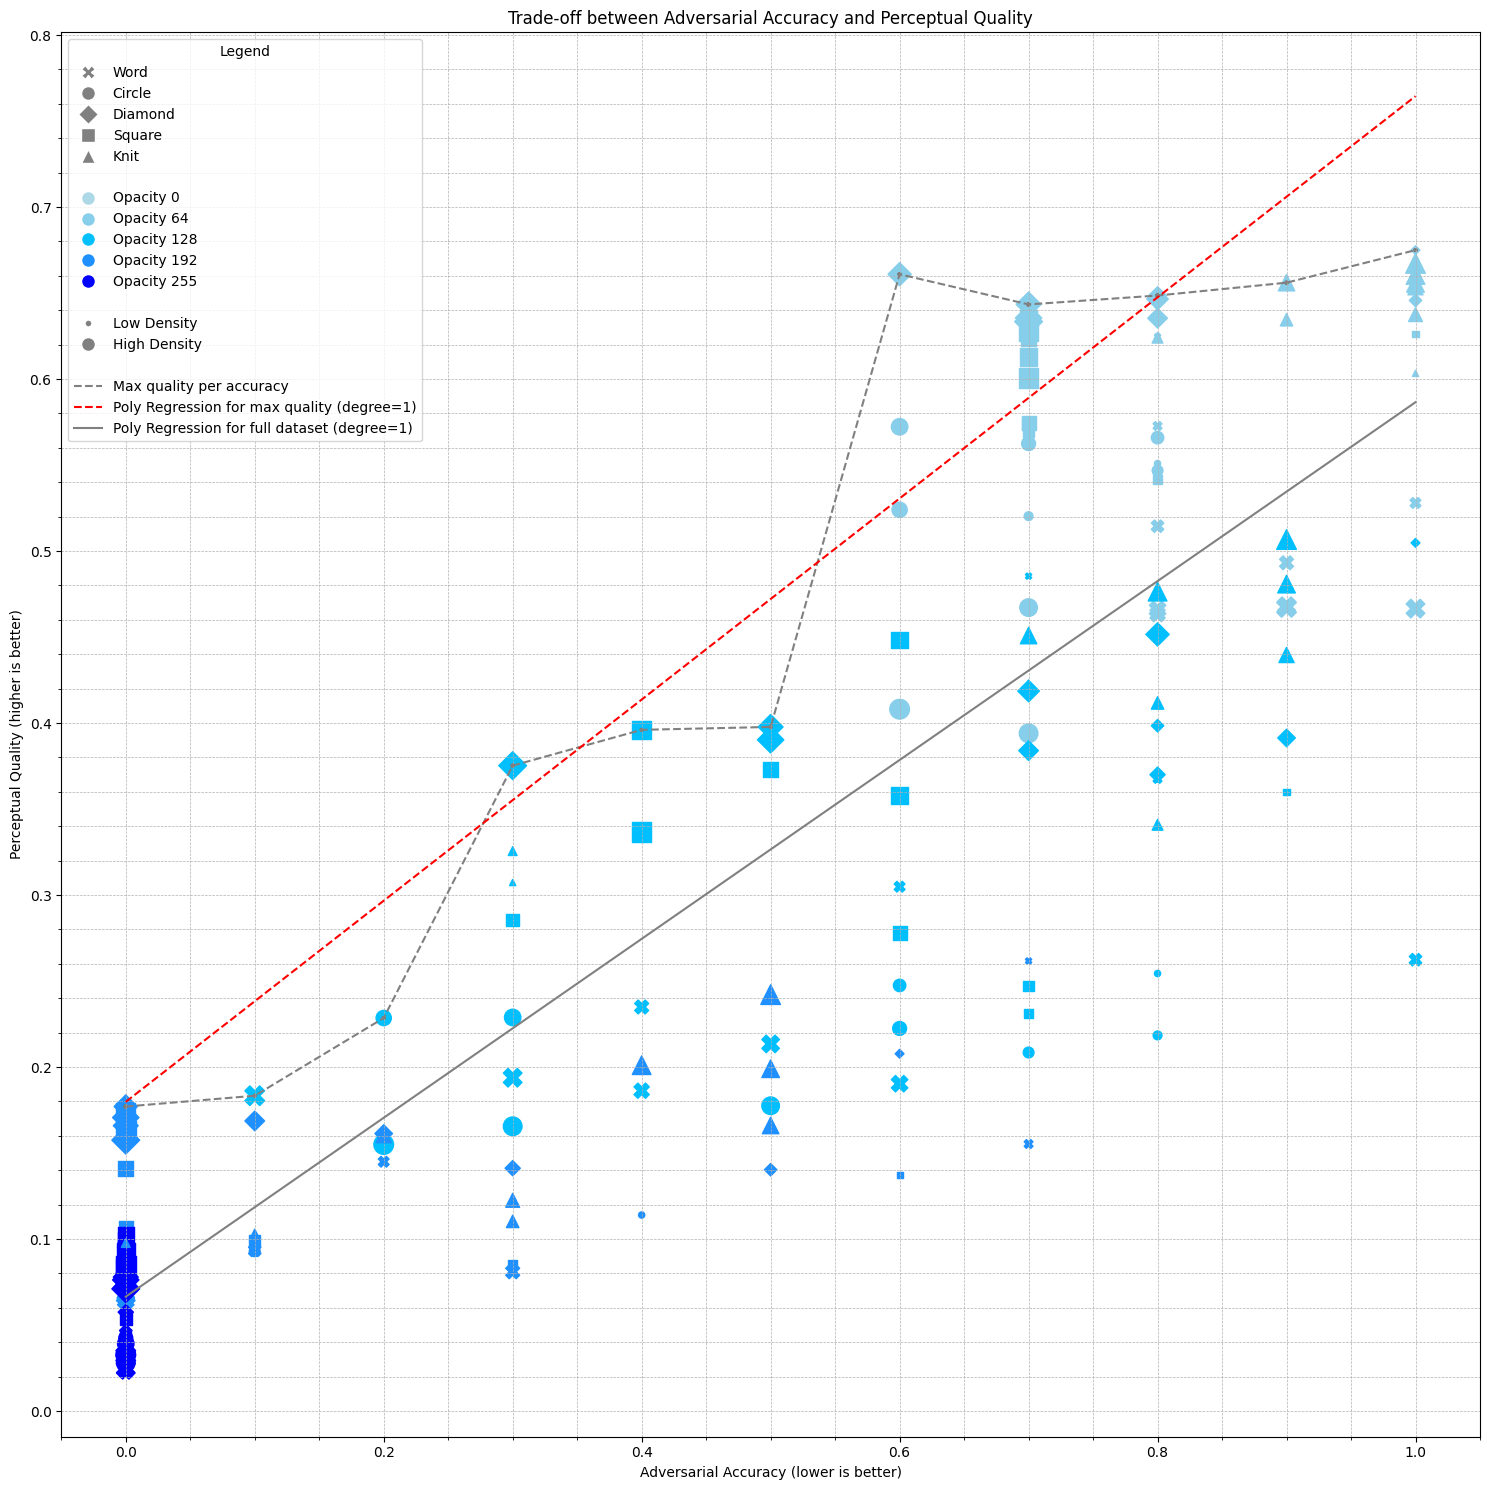
\includegraphics[width=1\columnwidth]{figures/tradeoff-1.png}
	\caption{Trade-off between accuracy and perceptual quality for the strongest masks.}
	\label{fig:tradeoff-1}
\end{figure}

Our second grid search, which combined FGSM perturbations with the masks, revealed some interesting insights. We found that combining perturbations with the masks generally led to worse results. The best results were obtained using the diamond mask with FGSM disabled, a density of 50 and opacities of 150 or 170. This further validated our previous findings and hinted that FGSM should be used with caution when combined with masks. Figure \ref{fig:tradeoff-2} shows the trade-off between accuracy and perceptual quality for the diamond mask combined with different opacities, densities and perturbation settings.

\begin{figure}
	\centering
	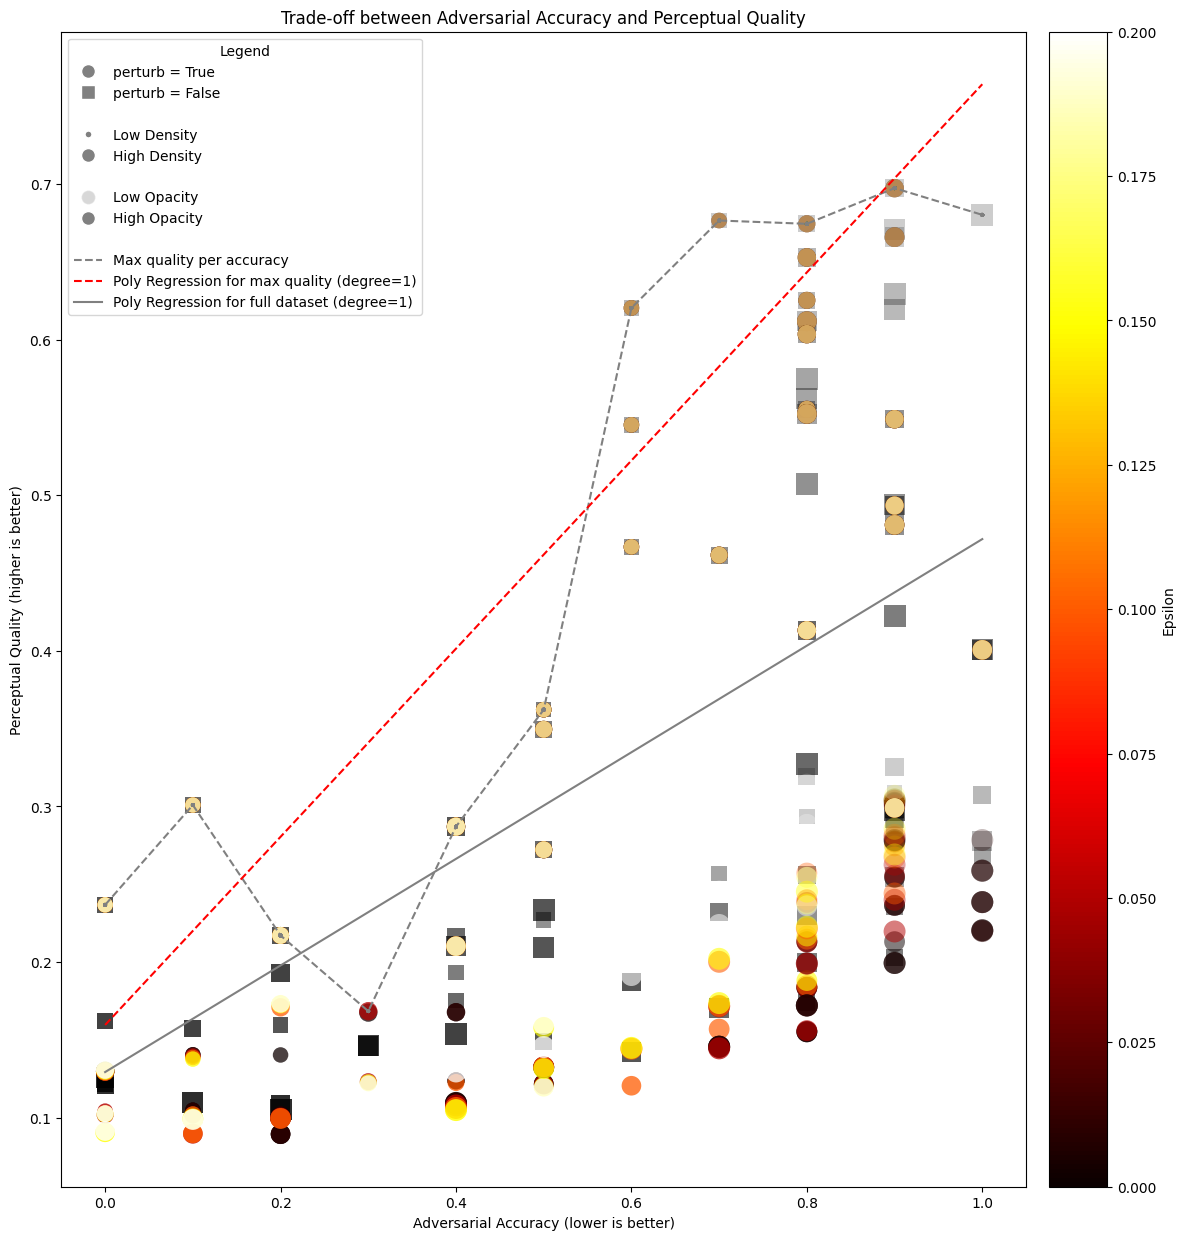
\includegraphics[width=1\columnwidth]{figures/tradeoff-2.png}
	\caption{Trade-off between accuracy and perceptual quality for the strongest masks.}
	\label{fig:tradeoff-2}
\end{figure}

While these results are not representative of the entire dataset or model space, they provide a good starting point for our experiments. We can conclude not to use perturbations with the masks. These initial findings also helped us identify the best configurations in opacity and density, to be used in the subsequent experiments. The final configurations of each mask are shown in figure \ref{fig:hcaptchacombined}.

\subsection{Results}

In our first set of experiments, we aimed to achieve two main objectives. First, we quantified the drop in top-1 and top-5 accuracy when various filters were applied to input images. Second, we compared the resilience of different model architectures to these adversarial examples.

\paragraph{Mask Generalizability.}

We assess how the rank of the correct class shifts when we apply the masks by checking the rank (position after sorting) of the ground-truth class before and after masking an image. Additionally, we evaluate the perceptual quality of the images. We then calculate the average change in rank across different models and images and present the findings for each mask and opacity combination. 

The results of our experiment are visualized in Figure~\ref{fig:accpercept} and summarized in Table~\ref{tab:generalizability}. The figure shows a clear trend in the trade-off between adversarial effectiveness and perceptual quality. The plot highlights an inverse relationship between these two factors, as indicated by the polynomial regression curve of degree 1. This relationship suggests that as the effectiveness of the adversarial attack increases (lower $\Delta$ Accuracy Rank), the perceptual quality of adversarial examples tends to decrease. While this is somewhat expected, we do see instances where there's a significant drop in rank (>10) while maintaining relatively high perceptual quality (>0.4).

The different mask types (circle, square, diamond and knit) and opacity levels show a range of performance across this trade-off spectrum. The scatter plot highlights clusters of points for each mask type, with some masks consistently striking a better balance between attack effectiveness and perceptual quality. Most importantly, these geometric pattern masks generalize well across state-of-the-art models.

\begin{figure}
	\centering
	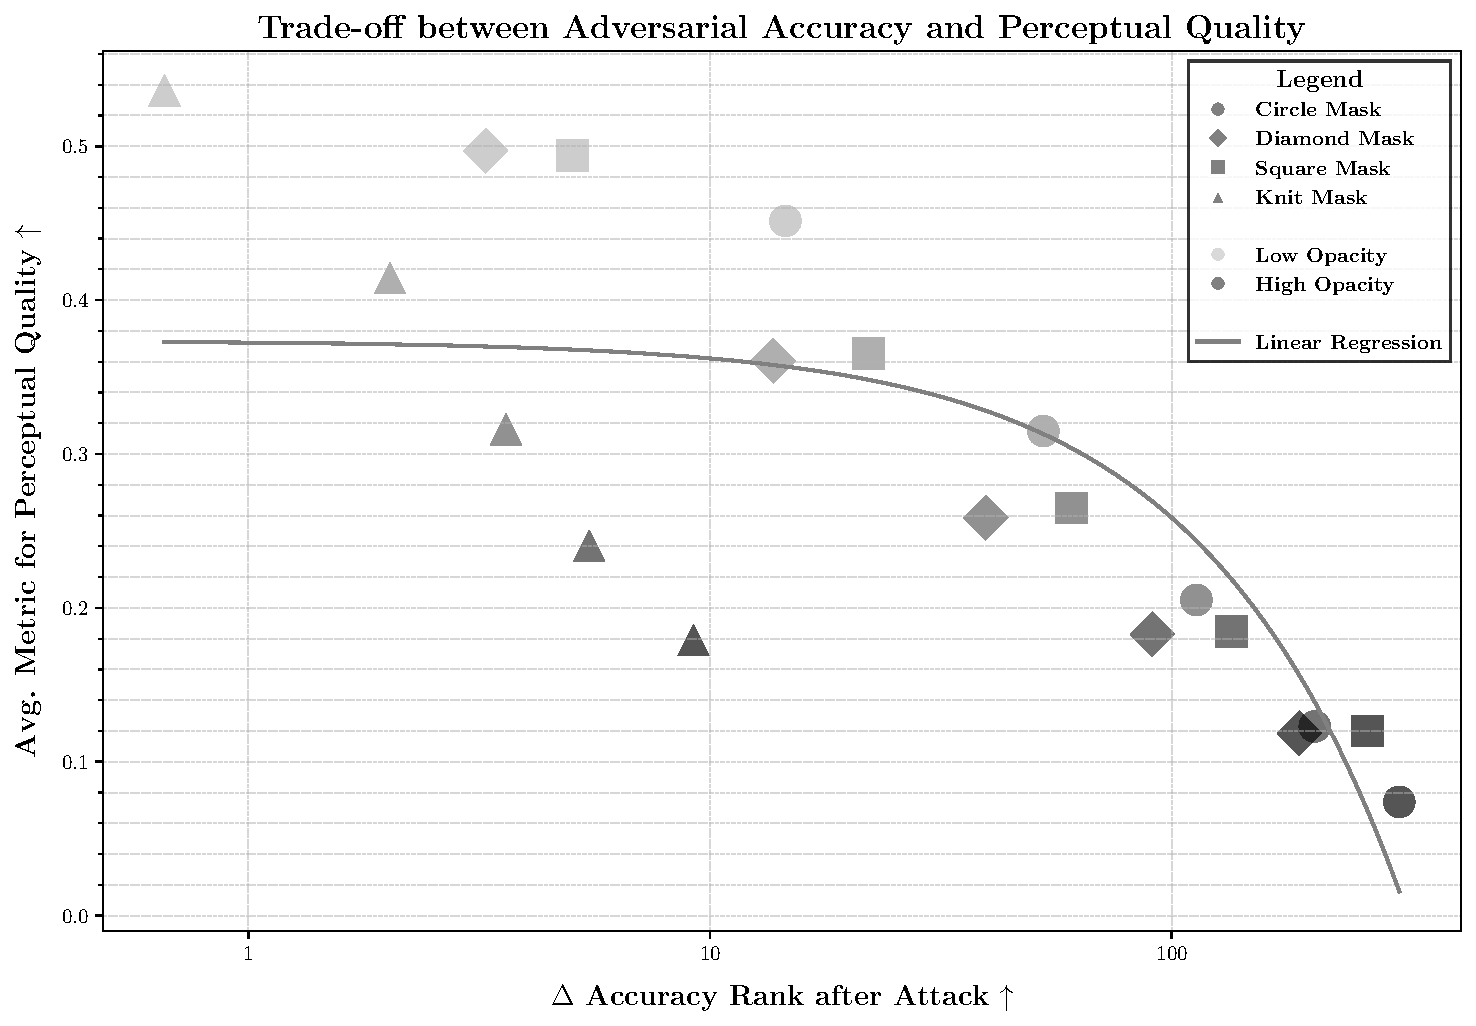
\includegraphics[width=1\columnwidth]{figures/eval_cls_generalizability.pdf}
	\caption{Accuracy vs. Perceptual Quality Trade-off}
	\label{fig:accpercept}
\end{figure}

\begin{table}[h]
    \centering
    \begin{tabular}{rlrrr}
        \toprule
        Opacity & Mask & $\Delta$ Acc Rank & Quality & Score \\
        \midrule
        \multirow{4}{*}{50}
            & Circle & -14.57 & 0.45 & 15.02 \\
            & Diamond & -3.27 & 0.50 & 3.76 \\
            & Knit & -0.66 & 0.54 & 1.19 \\
            & Square & -5.04 & 0.49 & 5.54 \\
        \midrule
        \multirow{4}{*}{80}
            & Circle & -52.72 & 0.31 & 53.03 \\
            & Diamond & -13.72 & 0.36 & 14.08 \\
            & Knit & -2.03 & 0.41 & 2.44 \\
            & Square & -22.01 & 0.37 & 22.37 \\
        \midrule
        \multirow{4}{*}{110}
            & Circle & -113.07 & 0.21 & 113.27 \\
            & Diamond & -39.55 & 0.26 & 39.81 \\
            & Knit & -3.62 & 0.32 & 3.93 \\
            & Square & -60.57 & 0.27 & 60.84 \\
        \midrule
        \multirow{4}{*}{140}
            & Circle & -203.89 & 0.12 & 204.01 \\
            & Diamond & -90.79 & 0.18 & 90.97 \\
            & Knit & -5.47 & 0.24 & 5.71 \\
            & Square & -134.75 & 0.18 & 134.94 \\
        \midrule
        \multirow{4}{*}{170}
            & Circle & -310.80 & 0.07 & 310.88 \\
            & Diamond & -188.92 & 0.12 & 189.04 \\
            & Knit & -9.21 & 0.18 & 9.39 \\
            & Square & -264.90 & 0.12 & 265.02 \\
        \bottomrule
    \end{tabular}
    \vspace*{0.1cm}
    \caption{Generalizability of Masks}
    \label{tab:generalizability}
\end{table}
	
\paragraph{Model Robustness.}

Finally, we evaluated the robustness of different models to our generated geometric masks. We measured the change in top-1 and top-5 accuracy for each model when presented with adversarial examples. The results are summarized in Table~\ref{tab:drop-acc1} and Table~\ref{tab:drop-acc5} for top-1 and top-5 accuracy, respectively. A negative value indicates an improvement in accuracy, while a positive value indicates a decrease. Larger values indicate a stronger effect of the adversarial examples.

There are many possible interpretations of these results. For example, the circle masks, contrary to our initial hyperparameter search, seem to be the most effective at reducing accuracy across all models and opacities. The knit mask, on the other hand, has a much smaller impact on accuracy.

\begin{table}[h]
	% this was accidentally mislabeled as subset-500 by andreas in the paper - it's actually the full imagenet dataset
	% see: https://github.com/ETH-DISCO/advx-bench/blob/main/analysis/4-eval_cls_modelperf.ipynb

    \setlength{\tabcolsep}{2pt}
    \tiny
    \centering
    \begin{minipage}{0.48\textwidth}
        \centering

        \begin{tabular}{ll|rrrrr}
			\multicolumn{2}{c|}{} & \multicolumn{5}{c}{Opacity} \\
			Model & Mask &  19\% & 31\% & 43\% & 54\% & 66\% \\
			\midrule
			\multirow{4}{*}{ConvNeXt} & Circle & 13.0  & 33.6  & 51.2  & 64.6  & 69.2  \\
			& Diamond & 4.8  & 13.6  & 31.8  & 49.6  & 64.6  \\
			& Knit & 2.2  & 3.2  & 8.0  & 11.4  & 18.0  \\
			& Square & 6.8  & 18.4  & 36.4  & 52.0  & 65.6 \\\midrule
			\multirow{4}{*}{EVA01} & Circle & 7.2  & 15.4  & 33.0  & 49.2  & 65.0  \\
			& Diamond & 2.6  & 8.6  & 19.6  & 33.0  & 54.8  \\
			& Knit & 1.2  & 1.2  & 4.4  & 6.6  & 10.6  \\
			& Square & 4.2  & 9.0  & 17.4  & 31.4  & 55.8 \\\midrule
			\multirow{4}{*}{EVA02} & Circle & 9.4  & 19.0  & 31.4  & 50.4  & 63.8  \\
			& Diamond & 2.4  & 5.6  & 10.6  & 19.0  & 38.0  \\
			& Knit & 2.8  & 4.8  & 5.2  & 6.8  & 8.8  \\
			& Square & 6.8  & 12.4  & 20.8  & 37.4  & 61.8 \\\midrule
			\multirow{4}{*}{ResNet} & Circle & 31.0  & 54.6  & 60.0  & 62.4  & 63.4  \\
			& Diamond & 13.2  & 31.6  & 50.4  & 59.4  & 62.2  \\
			& Knit & 5.0  & 11.2  & 14.4  & 19.4  & 27.6  \\
			& Square & 15.2  & 38.8  & 56.0  & 62.2  & 63.4 \\\midrule
			\multirow{4}{*}{ViT-H-14} & Circle & 5.8  & 20.6  & 48.2  & 70.8  & 80.2  \\
			& Diamond & 2.0  & 5.4  & 15.2  & 34.4  & 61.8  \\
			& Knit & 1.6 & 2.4  & 2.8  & 6.2  & 8.0  \\
			& Square & 3.2  & 9.6  & 25.0  & 54.2  & 77.2  \\
        \end{tabular}
        \vspace*{0.1cm}
        \caption{Change of Acc@1 in [\%].}
        \label{tab:drop-acc1}
        
    \end{minipage}%
    \hfill
    \begin{minipage}{0.48\textwidth}
        \centering

        \begin{tabular}{ll|rrrrr}
            \multicolumn{2}{c|}{} & \multicolumn{5}{c}{Opacity} \\
            Model & Mask &  19\% & 31\% & 43\% & 54\% & 66\% \\
            \midrule
            \multirow{4}{*}{ConvNeXt} & Circle & 7.60 & 29.60 & 54.80 & 73.40 & 85.00 \\
             & Diamond & 2.60 & 8.80 & 24.20 & 51.40 & 71.60 \\
             & Knit & 1.80 & 2.20 & 4.60 & 7.80 & 13.20 \\
             & Square & 4.80 & 13.20 & 28.80 & 54.80 & 76.80 \\\midrule
            \multirow{4}{*}{EVA01} & Circle & 4.80 & 14.00 & 27.80 & 50.60 & 75.40 \\
             & Diamond & 2.40 & 6.60 & 14.80 & 31.00 & 57.60 \\
             & Knit & 1.40 & 2.80 & 4.60 & 6.20 & 8.00 \\
             & Square & 3.40 & 7.00 & 12.60 & 28.20 & 61.00 \\\midrule
            \multirow{4}{*}{EVA02} & Circle & 4.60 & 12.20 & 24.40 & 44.60 & 65.00 \\
             & Diamond & 1.40 & 3.60 & 6.60 & 14.80 & 34.80 \\
             & Knit & 0.40 & 0.40 & 1.80 & 3.20 & 4.80 \\
             & Square & 2.20 & 6.60 & 15.00 & 31.40 & 63.60 \\\midrule
            \multirow{4}{*}{ResNet} & Circle & 34.20 & 67.40 & 80.40 & 85.40 & 86.20 \\
             & Diamond & 12.20 & 28.80 & 56.00 & 75.60 & 85.00 \\
             & Knit & 4.40 & 8.00 & 10.20 & 15.00 & 20.80 \\
             & Square & 15.20 & 40.20 & 66.40 & 82.20 & 86.60 \\\midrule
            \multirow{4}{*}{ViT-H-14} & Circle & 2.60 & 16.20 & 46.00 & 77.60 & 90.80 \\
             & Diamond & 0.20 & 2.20 & 10.60 & 28.60 & 61.20 \\
             & Knit & -0.60 & 0.60 & 1.00 & 2.00 & 3.20 \\
             & Square & 1.40 & 6.40 & 18.60 & 50.20 & 82.80 
        \end{tabular}
        \vspace*{0.1cm}
        \caption{Change of Acc@5 in [\%].}
        \label{tab:drop-acc5}

    \end{minipage}
\end{table}

% 
% self-ensemble experiments
% 

\section{Self-Ensembled ResNet}

\subsection{Research Motivation}

The self-ensembled ResNet~\cite{fort2024ensemble}, as presented in the previous chapter, is a novel approach to enhancing adversarial robustness in deep learning models. It combines multi-resolution inputs with dynamic self-ensembling of predictions from intermediate layers of the neural network. The multi-resolution input strategy involves feeding the model multiple versions of an image at different resolutions, inspired by biological mechanisms like eye saccades, which enhances robustness by forcing the network to process diverse representations simultaneously. The self-ensembling aspect leverages the inherent robustness of intermediate layer predictions, which are less affected by adversarial attacks targeting the final classifier. These predictions are aggregated using a consensus algorithm called ``CrossMax'', inspired by Vickrey auctions, which dynamically selects consistent outputs across layers:

\begin{minted}[fontsize=\footnotesize]{python}
def get_cross_max_consensus_logits(outputs: torch.Tensor, k: int) -> torch.Tensor:
    # subtract the max per-predictor over classes
    Z_hat = outputs - outputs.max(dim=2, keepdim=True)[0]
    # subtract the per-class max over predictors
    Z_hat = Z_hat - Z_hat.max(dim=1, keepdim=True)[0]
    # get highest k values per class
    Y, _ = torch.topk(Z_hat, k, dim=1)
    # get the k-th highest value per class
    Y = Y[:, -1, :]
    assert Y.shape == (outputs.shape[0], outputs.shape[2])
    assert len(Y.shape) == 2
    return Y
\end{minted}

Architecturally, what makes this approach special is its ability to use a single ResNet model to create a ``self-ensemble'' by decoupling and aggregating predictions from different layers. This eliminates the need for multiple independent models while still achieving ensemble-like robustness. Additionally, the use of multi-resolution inputs and stochastic augmentations reduces the attack surface for adversarial perturbations.

We also noticed a gap in reproducibility studies for this model, due to its recency and complexity. This was an additional incentive for us to explore this approach further.

\subsection{Experimental Setup}

\paragraph{Hyperparameter Search (on custom model).}

Approximately two months following the publication of the paper, the authors released a notebook detailing their preprocessor (including saccading, jitter and nature-imitating noise, ...), architecture and training pipeline. We opted to reconstruct the architecture independently\footnote{Credits to Andreas Plesner.} and implemented the CrossMax consensus algorithm. Our hyperparameter search encompassed the following parameters: dataset (CIFAR10, CIFAR100), learning rate (1e-1, 1e-4, 1e-5, 1.7e-5, 1e-6, 1e-7), number of epochs (4, 8, 16) and CrossMax $k$ (2, 3). We employed a grid search methodology to identify the optimal settings for our custom model.

We found the best results with a learning rate of 1e-4, running for 16 epochs and setting CrossMax $k$ to 2. Interestingly, running more epochs only bumped up performance by less than 1\%, so we stuck with 16 epochs. For CrossMax $k$, 2 was the sweet spot for both datasets, although CIFAR10 showed a tiny edge with $k=3$ by just 0.1\%. These results are visualized in Figure~\ref{fig:se-hyperparams}. When the authors later shared parts of their implementation and hyperparameters, our findings were in line with theirs, except for slight differences in the learning rate (3.3e-5 vs 1e-4) and the number of epochs (6 vs 16). We believe these differences to be due to the computational limits they set for their experiments.

\begin{figure}
	\centering
	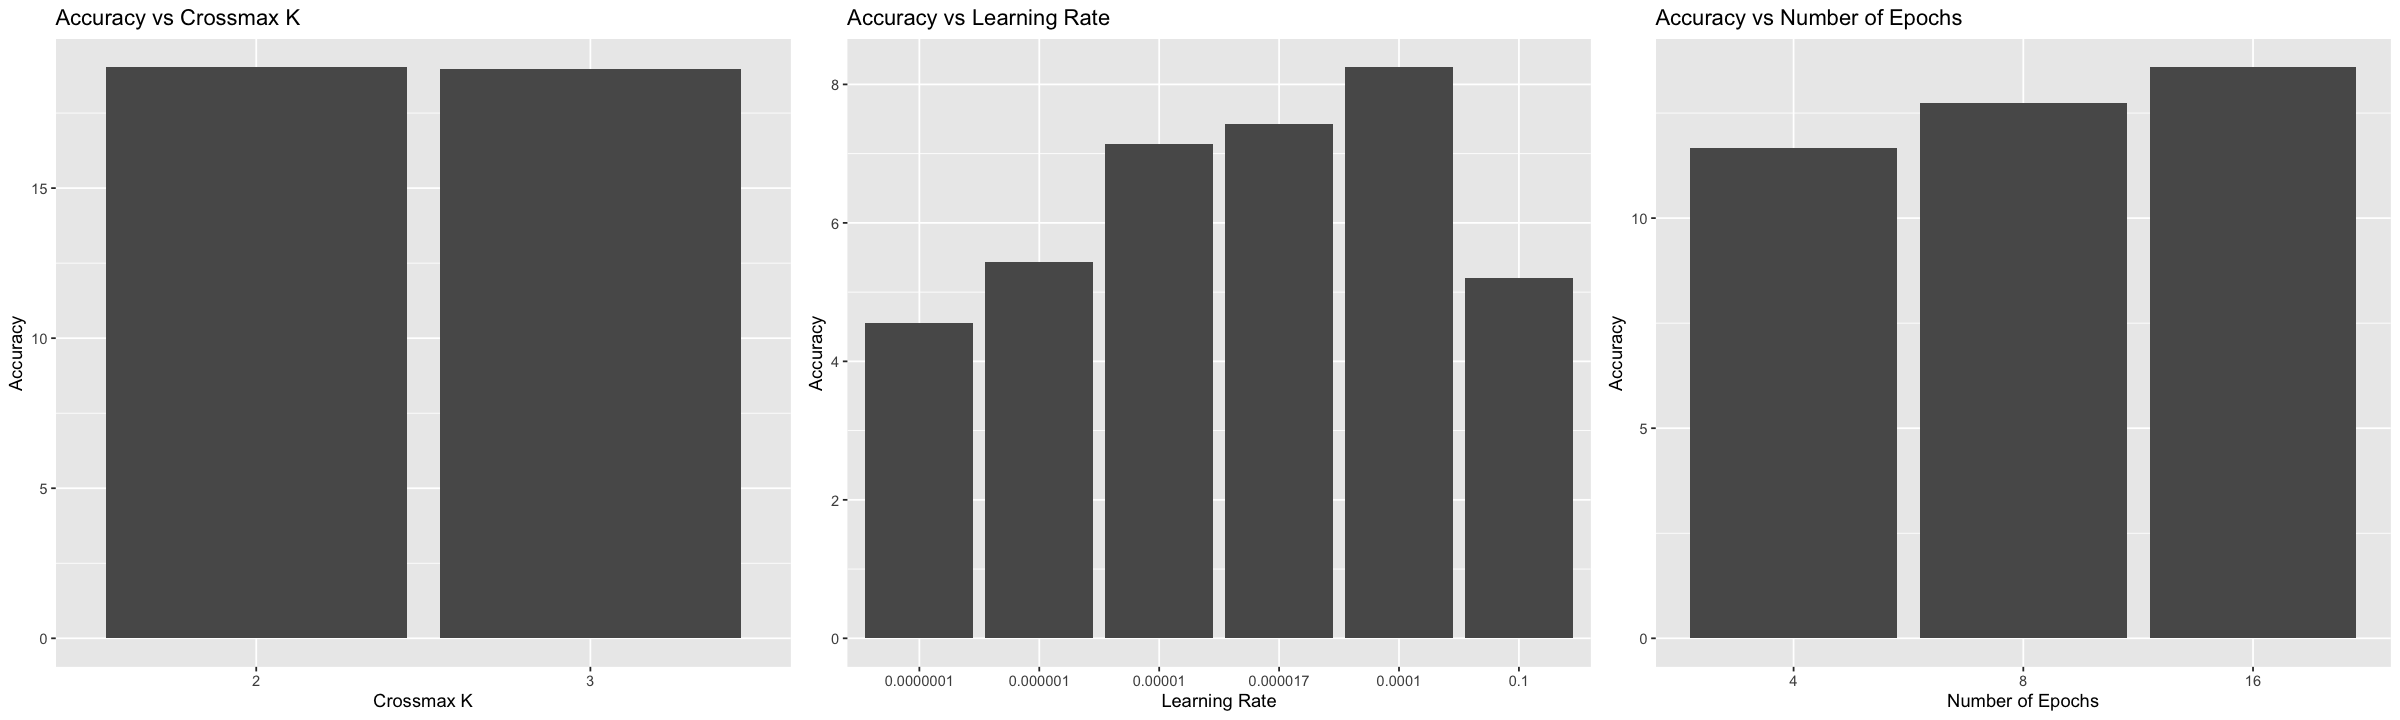
\includegraphics[width=1\columnwidth]{figures/self-ensemble-hyperparams.png}
	\caption{Hyperparameter search for the self-ensembled ResNet.}
	\label{fig:se-hyperparams}
\end{figure}


\subsection{Results}


\bigskip
\bibliographystyle{IEEEtran}
\bibliography{references}

% \appendix
% \chapter{Appendix}

\end{document}
